%%%%%%%%%%%%%%%%%%%%%%% preamble %%%%%%%%%%%%%%%%%%%%%%%%%%%
\documentclass[10pt,letterpaper]{article}
\usepackage{opex3}
\usepackage{epstopdf}
\usepackage{color}
\usepackage{amsmath}
\usepackage{amssymb}
\usepackage{graphicx}
\usepackage{multirow}
\usepackage{caption}
\usepackage{subcaption}
\usepackage{floatrow}
\newfloatcommand{capbtabbox}{table}[][\FBwidth]
\usepackage{blindtext}
\usepackage{cite}
\usepackage{array}


\makeatletter
\newcommand*{\rmnum}[1]{\expandafter\@slowromancap\romannumeral #1@}
\makeatother
\newcommand{\vm}[1]{{\bf{#1}}}
\newcommand{\vecttwo}[2]
{
	\left[
		\begin{eqnarray*}
		#1\\
		#2
		\end{eqnarray*}
	\right]
}
\newcommand{\vectthree}[3]
{
	\left[
		\begin{eqnarray*}
		#1\\
		#2\\
		#3
		\end{eqnarray*}
	\right]
}

%%%%%%%%%%%%%%%%%%%%%%% begin %%%%%%%%%%%%%%%%%%%%%%%%%%%%%%
\begin{document}

%%%%%%%%%%%%%%%%%% title page information %%%%%%%%%%%%%%%%%%
\title{Performance of Color Shift Keying under non-linear system model and illumination constraints}

\author{Pankil M. Butala$^{1,2}$, Hany Elgala$^{1,3}$ and Thomas D.C. Little$^{1,4}$}

\address{$^{1}$Multimedia Communication Laboratory and Smart Lighting Engineering Research Center\\
Boston University, Boston, MA 02215, USA\\
\{$^2$pbutala,$^3$helgala,$^4$tdcl\}@bu.edu}

% \homepage{http:...} %% author's URL, if desired

%%%%%%%%%%%%%%%%%%% abstract and OCIS codes %%%%%%%%%%%%%%%%
%% [use \begin{abstract*}...\end{abstract*} if exempt from copyright]

\begin{abstract}
The IEEE 802.15.7 standard defines specifications for short-range wireless optical communication using visible light. The standard specifies color shift keying (CSK) as the preferred modulation scheme for indoor optical wireless communications when simultaneously providing illumination. CSK is indicated in standard with 7 color bands and 9 color band combinations using distinct LED colors. This article studies the performance of M-ary CSK under the linear system model as specified in the standard, but also when nonlinearities are considered as dictated by the difference between human perception and radiant flux and the inherent characteristics implied by modeling in the CIE color coordinate system. It is shown that these nonlinearities introduce performance penalties of more than 15dB, 10dB, and 5dB for M=4, 8, and 16-CSK respectively. Additionally, the requirement to maintain a target illumination intensity in a practical lighting system constrains the average radiant flux available for communication using the different color band combinations. The analysis shown introduces a luminous-signal-to-noise ratio (LSNR) metric and compares performance of different color band combinations emitting different radiant fluxes for M-ary CSK as a result of user defined target illumination constraints.
\end{abstract}

\ocis{(060.2605) Free-space optical communication, (060.4080) Modulation, (060.4510) Optical communications} 
% REPLACE WITH CORRECT OCIS CODES FOR YOUR ARTICLE, MINIMUM OF TWO; Avoid using the OCIS codes for “General” or “General science” whenever possible.

%%%%%%%%%%%%%%%%%%%%%%% References %%%%%%%%%%%%%%%%%%%%%%%%%
\begin{thebibliography}{99}
\bibitem{cis14a} ``{Cisco visual networking index: forecast and methodology, 2013-2018},'' (2014).
%\bibitem{rah11a} Rahaim et al ''{A hybrid Radio Frequency and broadcast Visible Light Communication system},'' Globecom Workshops, IEEE 792-796 (2011).
\bibitem{rah15a} M. Rahaim and T. Little, ``{Towards Practical Integration of Dual-Use VLC within 5G Networks},'' to appear in IEEE Wireless Comm. (2015).
\bibitem{gru08b} J. Grubor, S. Randel, K-D Langer and J.W. Walewski, ``{Broadband Information Broadcasting Using LED-Based Interior Lighting},'' J. Lightwave Tech. {\bf 26}(24), 3883--3892 (2008).
\bibitem{min08a} H. Minh, D. O'Brien, G. Faulkner, L. Zeng, K. Lee, D. Jung and Y. Oh, ``{High-Speed Visible Light Communications Using Multiple-Resonant Equalization},'' IEEE Photon. Lett. {\bf 20}(14), 1243--1245 (2008).
\bibitem{arm09a} J. Armstrong ``{OFDM for Optical Communications},'' J. Lightwave Tech. {\bf 27}(3), 189-204 (2009).
\bibitem{but14b} P. Butala, H. Elgala and T. Little, ``{Sample indexed spatial orthogonal frequency division multiplexing},'' Chin. Opt. Lett. {\bf 12}(9), 090602 (2014)
\bibitem{cskxy} A. Yokoi, J. Son and T. Bae, ``{CSK constellation in all color band combinations},'' {https://mentor.ieee.org/802.15/dcn/11/15-11-0247-00-0007-csk-constellation-in-all-color-band-combinations.pdf} (2011).
\bibitem{but12a} P. Butala, J. Chau and T. Little, ``{Metameric modulation for diffuse visible light communications with constant ambient lighting},'' Intl. Workshop on Opt. Wireless Comm. (IWOW), 1-3 (2012).
\bibitem{ieee802.15.7} ``{IEEE Standard for Local and Metropolitan Area Networks--Part 15.7: Short-Range Wireless Optical Communication Using Visible Light},'' (2011).
\bibitem{raj12a} S. Rajagopal, R.D. Roberts and S-K Lim, ``{IEEE 802.15.7 visible light communication: modulation schemes and dimming support},'' IEEE Comm. Mag. {\bf 50}(3), 72-82 (2012).
\bibitem{sin13a} R. Singh, T. O'Farrell and J.P.R. David, ``{Performance evaluation of IEEE 802.15.7 CSK physical layer},'' Globecom Workshops, IEEE 1064-1069 (2013).

%\bibitem{gallo99} K. Gallo and G. Assanto, ``All-optical diode based on second-harmonic generation in an asymmetric waveguide,'' \josab {\bf 16}(2), 267--269 (1999).
%{\bf volume}(issue)

\end{thebibliography}

%%%%%%%%%%%%%%%%%%%%%  Introduction  %%%%%%%%%%%%%%%%%%%%%%%
\section{Introduction}\label{sINTR}

Rapid growth of portable computing devices is severely increasing demand for wireless data access \cite{cis14a}. Studies indicate current infrastructure cannot satisfy this demand. Thus there is critical need to exploit additional spectrum to augment wireless infrastructure. On the other hand, solid state device industry has made great advances in engineering energy efficient light emitting diode (LED). Lighting manufacturers are quickly replacing traditional lighting sources with efficient LEDs to provide illumination. This has created an opportunity to exploit the visible spectrum (380nm-780nm) used for indoor illumination and provide concurrent opportunistic wireless connectivity. 

Under the above model, luminaires need to service dual missions of illumination and wireless access points. A practical system would exploit the visible spectrum in coordination with the radio frequency (RF) spectrum to form a heterogeneous system. The visible spectrum can be used to augment the down-link whenever a good link is available. In applications where using the visible spectrum for up-link is not user friendly, the system can rely on existing RF infrastructure \cite{rah15a}.

Visible light communication (VLC) uses intensity-modulation direct-detection (IM/DD) for wireless data transfer. Capacity of such a system using LEDs as transmitters is usually limited by their bandwidth. Typical illumination grade LEDs are phosphor converted white LEDs with a bandwidth of about 2 MHz \cite{gru08b}. Techniques to enhance the bandwidth up to and beyond 20 MHz have been documented in references \cite{gru08b,min08a}. 

Different modulation schemes used in conjunction with IM/DD have been proposed for use with VLC. Optical orthogonal frequency division multiplexing schemes provide high spectral efficiency for a single-input single-output (SISO) VLC channel \cite{arm09a}. To achieve better spectral efficiency, multiple-input multiple-output (MIMO) techniques exploiting dimensions of space and color have also been documented \cite{but14b,cskxy,but12a}.

The IEEE standard for short-range wireless optical communication using visible light \cite{ieee802.15.7} specifies Color Shift Keying (CSK) as the modulation technique of choice under the physical layer (PHY) \rmnum{3} specifications. The standard outlines different PHY \rmnum{3} configurations to achieve up to 96 Mb/s data rate while maintaining target illumination. The standard outlines M-ary CSK under a linear system model. Reference \cite{raj12a} provides an overview of modulation and dimming techniques specified within the standard while reference \cite{sin13a} studies select color bands for CSK.

This article studies M-ary CSK for all color band combinations as outlined in the standard and then extends the study to include practical implementation constraints -- a) Non-linearity introduced by illumination to radiant flux transformation and vice versa and b) User defined target illumination intensity level. In the process, a new metric - luminous-signal-to-noise ratio (LSNR) is introduced to compare performance of different signaling schemes at a target illumination intensity level.

An overview of color shift keying modulation technique is provided in Section \ref{sCSK}. The linear CSK model as described in standard \cite{ieee802.15.7} is then outlined in Section \ref{sCSKL}. CSK performance considerations in a practical scenario due presence of non-linearity introduced by color to radiant flux transformation is considered in Section \ref{sCSKNL}. Section \ref{sCSKLSNR} introduces LSNR and CSK performance considerations due to practical illumination constraints. Some conclusions are then drawn in Section \ref{sCONC}.

%%%%%%%%%%%%%%%%%%  Color Shift Keying  %%%%%%%%%%%%%%%%%%%%
\section{Color Shift Keying}\label{sCSK}
LED based luminaires are energy efficient and are thus being widely adopted in indoor spaces to provide illumination. In order to dynamically control the illumination spectrum, luminaires contain multiple elements of at least three colors of LEDs. A number of different spectra can be generated by mixing different ratios of radiant flux emitted from the multiple LEDs comprising a luminaire. Each spectrum looks like a different color to human eye.

Any spectral power distribution (SPD) within the visible range of electromagnetic spectrum can produce a stimulus when incident on the sensors (rod and cones) of human eye and has a color associated with it. This color is represented by its intensity, hue and saturation. While intensity is a measure of the total power comprising the SPD, hue and saturation are subjective parameters analogous to mean and spread of the wavelengths comprising the SPD and quantified by a chromaticity coordinate. The \textit{commission internationale de l'eclairage} (CIE) has specified the CIE 1931 XYZ color space (CS) that provides a mathematical model to represent the chromaticity of radiation in the visible range as a point in a 2-dimensional plane. Let a luminaire be comprised of three types of LEDs, namely LED$_{n}$; $n\in\{i,j,k\}$. The chromaticity of each LED can be represented by a coordinate (x$_{n}$,y$_{n}$) on the CS. When different intensities of radiant flux emitted by three types of LEDs are combined, the chromaticity coordinate of the resultant SPD will lie inside the triangle formed by vertices I (x$_{i}$,y$_{i}$), J (x$_{j}$,y$_{j}$) and K (x$_{k}$,y$_{k}$). 

\renewcommand{\arraystretch}{1.05}
\begin{figure}[b]
\begin{floatrow}
		\capbtabbox{
			\begin{tabular}{|c|c|c|c|c|}
			\hline
			\multirow{2}{*}{\textbf{CB$_{u}$}} & \textbf{Band} & \textbf{Center} & \multirow{2}{*}{\textbf{x}} & \multirow{2}{*}{\textbf{y}}\\
			 & \textbf{(nm)} & \textbf{(nm)} & & \\
			\hline
			CB$_{0}$ & 380 - 478 & 429 & 0.169 & 0.007\\
			\hline
			CB$_{1}$ & 478 - 540 & 509 & 0.011 & 0.733\\
			\hline
			CB$_{2}$ & 540 - 588 & 564 & 0.402 & 0.597\\
			\hline
			CB$_{3}$ & 588 - 633 & 611 & 0.669 & 0.331\\
			\hline
			CB$_{4}$ & 633 - 679 & 656 & 0.729 & 0.271\\
			\hline
			CB$_{5}$ & 679 - 726 & 703 & 0.734 & 0.265\\
			\hline
			CB$_{6}$ & 726 - 780 & 753 & 0.734 & 0.265\\
			\hline
			\multicolumn{5}{c}{ }
			\end{tabular}}
			{\caption{Color bands.}}
			\ffigbox{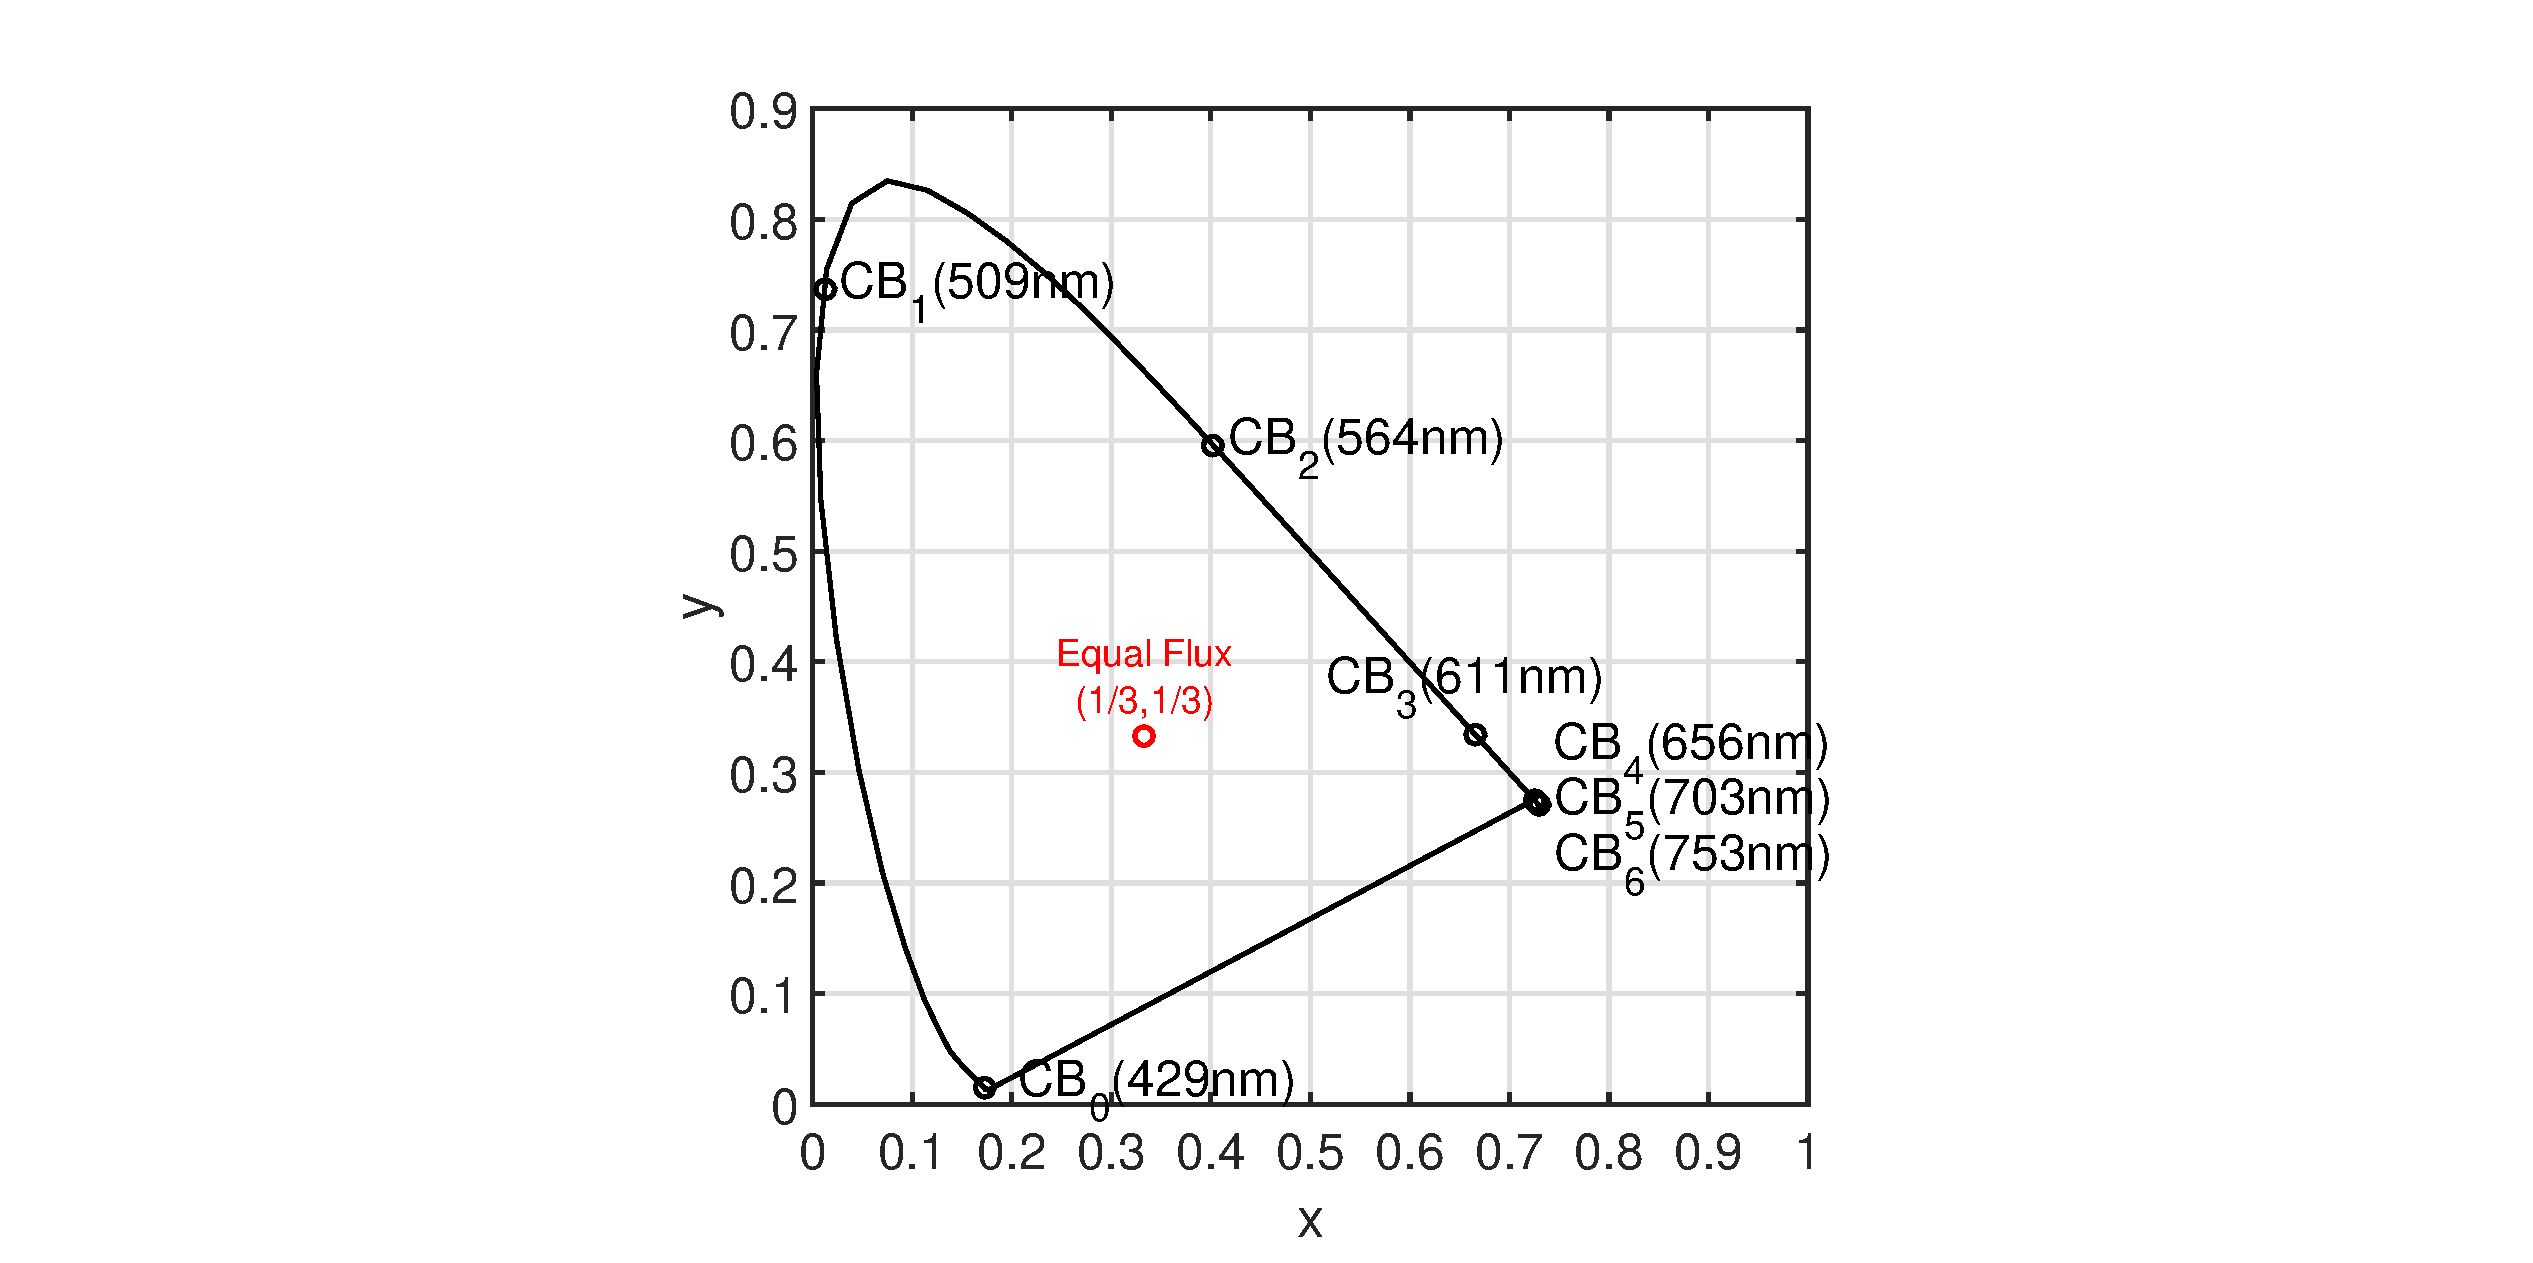
\includegraphics[trim={4.3in 0in 4.3in 0.5in}, clip=true, width=1.8in]{CBCcenters.eps}}
			{\caption{Color band centers.}}
	\end{floatrow}
\end{figure}
\renewcommand{\arraystretch}{1}

\begin{table}[b]
\centering
\begin{tabular}{|c|c|c|c|}
\hline
Color band combination & \multicolumn{3}{c|}{Color band '$u$' for CBC$_{v}$} \\
\cline{2-4}
\textbf{CBC$_{v}$} & \textbf{Band i} & \textbf{Band j} & \textbf{Band k} \\
\hline
CBC$_{1}$ & 6 & 2 & 0 \\
\hline
CBC$_{2}$ & 6 & 1 & 0 \\
\hline
CBC$_{3}$ & 5 & 2 & 0 \\
\hline
CBC$_{4}$ & 5 & 1 & 0 \\
\hline
CBC$_{5}$ & 4 & 2 & 0 \\
\hline
CBC$_{6}$ & 4 & 1 & 0 \\
\hline
CBC$_{7}$ & 3 & 2 & 0 \\
\hline
CBC$_{8}$ & 3 & 1 & 0 \\
\hline
CBC$_{9}$ & 2 & 1 & 0 \\
\hline
\end{tabular}
\caption{Color bands combinations as specified by the standard.}
\label{tCBC}
\end{table}

CSK is a modulation technique in which information is transmitted through changes in chromaticity coordinate. This can be achieved by varying the intensities of LED$_{n}$ over time depending on the information to transmit. In order to select LED$_{n}$, the standardized CSK implementation specifies 7 different color bands (CB$_{u}$); $0\leq u < 7$ as shown in Table 1. The color bands are obtained by splicing the visible spectrum range into 7 contiguous segments. Though not explicitly mentioned, it is assumed that SPD of each LED$_{n}$ must belong to a different sector enclosed by a color band and point (1/3,1/3). To study performance of CSK independent of specific LED characteristics, it is generally assumed that the chromaticity coordinate of LED belonging to a color band corresponds to the center wavelength of sector with CB$_{u}$ as illustrated in \figurename 1.

To realize CSK using 3 types of LEDs, the standard defines different sets of 3 color bands and calls each set a color band combination (CBC). The 3 different types of LEDs forming a CBC are ordered in a descending manner based on the center wavelength of the color band they belong to and each such band is called 'band i', 'band j' and 'band k' respectively. 9 such CBC$_{v}$; $1\leq v\leq 9$ are defined in the standard and are outlined in Table \ref{tCBC}. For the rest of this article, generalized notation CB$^{v}_{n}$ will be used to indicate color band $n\in\{i,j,k\}$ belonging to CBC$_{v}$. Using this notation CB$^{1}_{i}$ $\equiv$ CB$_{6}$ while CB$^{2}_{j}$ $\equiv$ CB$_{1}$ and so on.

For an M-ary CSK using CBC$_{v}$, the design rules to compute the 'M' different constellation points are provided in the standard and their values are outlined in \cite{cskxy}. Let C$^{v}_{n}\equiv$(x$^{v}_{n}$,y$^{v}_{n}$) be chromaticity coordinate corresponding to CB$^{v}_{n}$. Let C$_{m}\equiv$(x$_{m}$,y$_{m}$); $0\leq m <$ M be chromaticity coordinate corresponding to m$^{th}$ codeword. Then Table 3 outlines the design rules for computing the constellation points. C$^{v}_{n}$ can be looked up from Table \ref{tCBC} and Table 1. Using these values, remaining C$_{m}$ can then be computed using rules from Table \ref{tMCSK}. Normalized constellation design rules for M-ary CSK are illustrated in \figurename\ref{figConst}. Points I, J and K represent normalized coordinates for the n color bands comprising a CBC. 

CSK is implemented in conjunction with IM/DD over the optical channel. This channel can be modeled as a LTI AWGN and mathematically represented as in Eq.(\ref{eqCHNL})

\begin{equation}
	\vm{Y} = \vm{H}\vm{X} + \vm{W}
	\label{eqCHNL}
\end{equation}
where \vm{X} is an n$_{tx}$ dimensional vector containing transmit optical powers for each band n, \vm{H} is a n$_{rx}\times$n$_{tx}$ dimensional channel matrix, \vm{W} is a n$_{rx}$ dimensional noise vector and \vm{Y} is an n$_{rx}$ dimensional receive vector. Channel matrix \vm{H} includes the responsivities of the receive elements.

\begin{figure}[t]
	\centering
		\begin{subfigure}{0.32\textwidth}
		\centering
			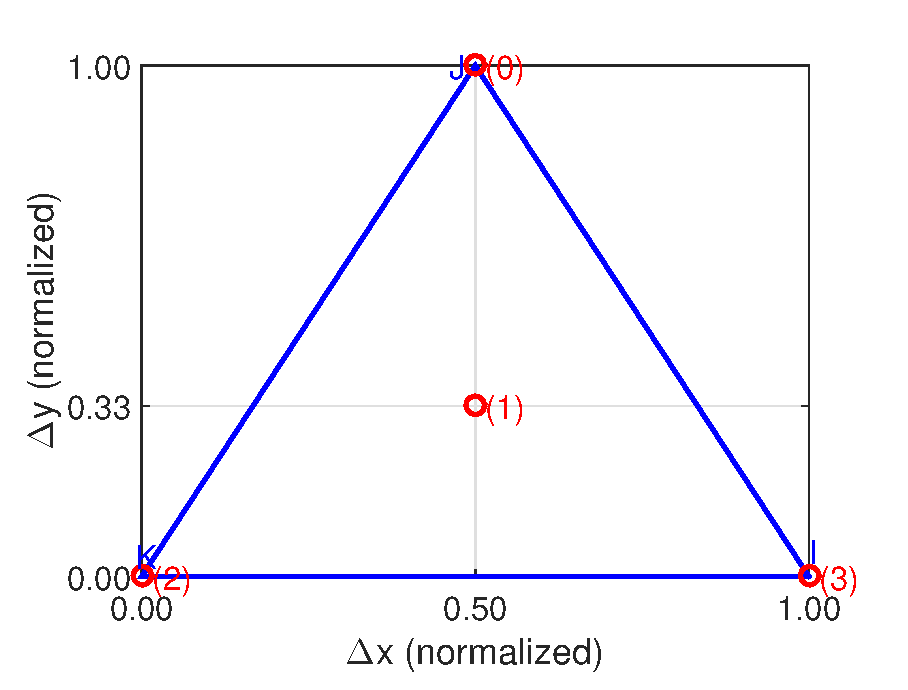
\includegraphics[trim={0.05in 0.0in 0.25in 0.2in}, clip=true, width=\textwidth]{CBCrules4.eps}
			\caption{4-CSK}
			\label{fig4Const}
		\end{subfigure}
		\hfill
		\begin{subfigure}{0.32\textwidth}
		\centering
			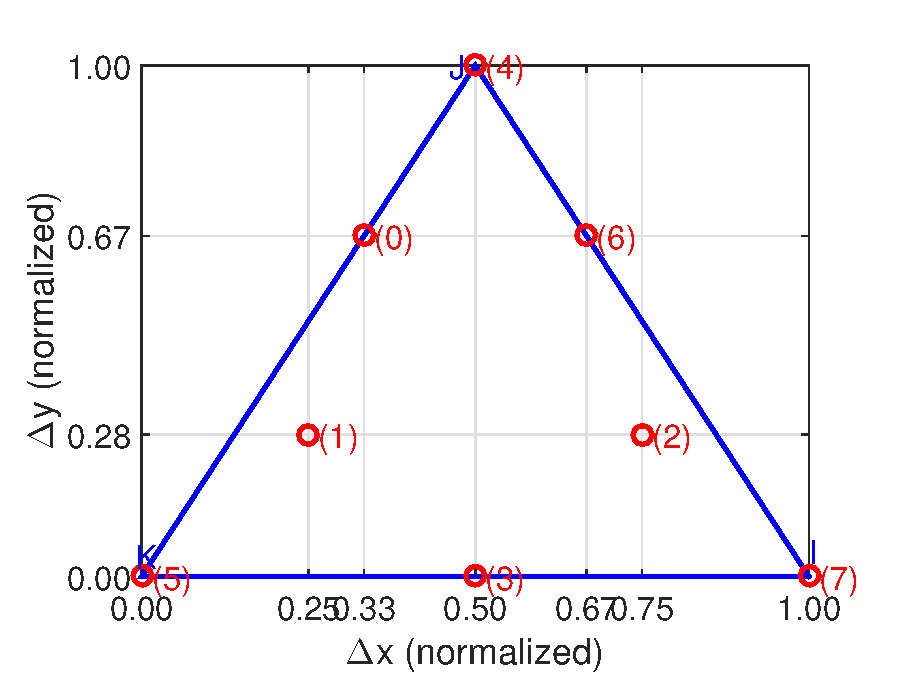
\includegraphics[trim={0.05in 0.0in 0.25in 0.2in}, clip=true, width=\textwidth]{CBCrules8.eps}
			\caption{8-CSK}
			\label{fig8Const}
		\end{subfigure}
		\hfill
		\begin{subfigure}{0.32\textwidth}
		\centering
			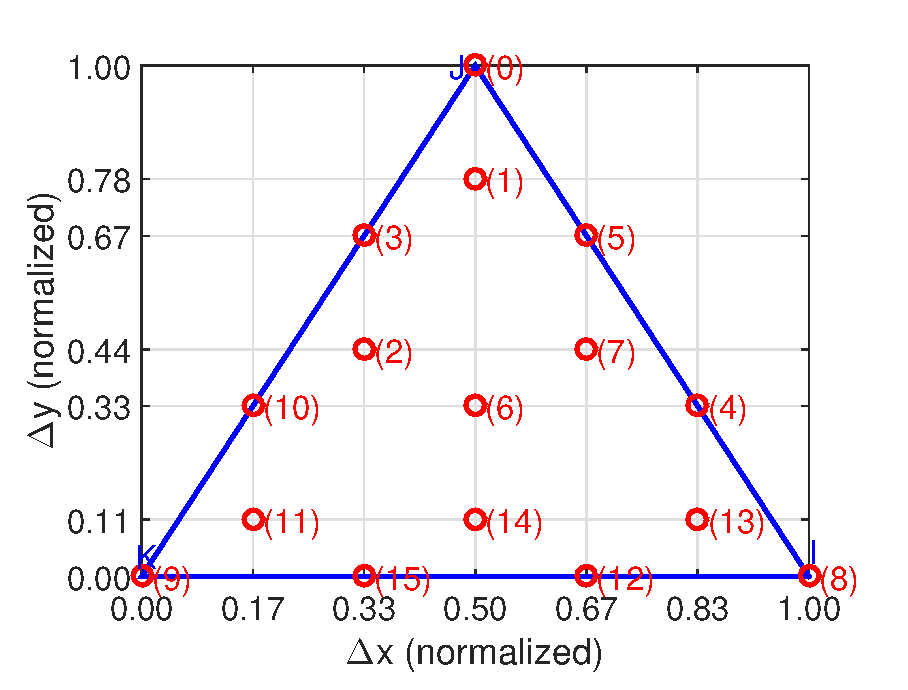
\includegraphics[trim={0.05in 0.0in 0.25in 0.2in}, clip=true, width=\textwidth]{CBCrules16.eps}
			\caption{16-CSK}
			\label{fig16Const}
		\end{subfigure}
	\caption{M-ary CSK (normalized) constellation design rules.}
	\label{figConst}
\end{figure}

\begin{table}[t]
\centering
\begin{tabular}{|c|c|c|c|}
\hline
\textbf{m} & \textbf{M = 4} & \textbf{M = 8} & \textbf{M = 16} \\
\hline
0 & C$^{v}_{j}$ & (2C$_{4}$+C$_{5}$)/3 & C$^{v}_{j}$\\
1 & (C$^{v}_{i}$+C$^{v}_{j}$+C$^{v}_{k}$)/3 & (2C$_{a}$+C$_{b}$)/3; C$_{a}$=(C$_{b}$+C$_{3}$+C$_{5}$)/3; C$_{b}$=(C$_{4}$+C$_{5}$)/2 & (C$_{0}$+C$_{3}$+C$_{5}$)/3 \\
2 & C$^{v}_{k}$ & (2C$_{a}$+C$_{b}$)/3; C$_{a}$=(C$_{b}$+C$_{3}$+C$_{7}$)/3; C$_{b}$=(C$_{4}$+C$_{7}$)/2 & (C$_{3}$+C$_{6}$+C$_{10}$)/3 \\
3 & C$^{v}_{i}$ & (C$_{5}$+C$_{7}$)/2 & (2C$_{0}$+C$_{9}$)/3 \\
\cline{2-2}
4 & & C$^{v}_{j}$ & (C$_{0}$+2C$_{8}$)/3 \\
5 & & C$^{v}_{k}$ & (2C$_{0}$+C$_{8}$)/3 \\
6 & & (2C$_{4}$+C$_{7}$)/3 & (C$_{0}$+C$_{8}$+C$_{9}$)/3 \\
7 & & C$^{v}_{i}$ & (C$_{4}$+C$_{5}$+C$_{6}$)/3 \\
\cline{3-3}
8 & & & C$^{v}_{i}$ \\
9 & & & C$^{v}_{k}$ \\
10 & & & (C$_{0}$+2C$_{9}$)/3 \\
11 & & & (C$_{9}$+C$_{10}$+C$_{15}$)/3 \\
12 & & & (2C$_{8}$+C$_{9}$)/3 \\
13 & & & (C$_{4}$+C$_{8}$+C$_{12}$)/3 \\
14 & & & (C$_{6}$+C$_{12}$+C$_{15}$)/3 \\
15 & & & (C$_{8}$+2C$_{9}$)/3 \\
\hline
\end{tabular}
\caption{Design rules to compute constellation points for M-CSK. Each row computes C$_{m}$ for m$^{th}$ codeword given CBC$_{v}$.}
\label{tMCSK}
\end{table}

In M-ary CSK, n$_{tx}=3$ types of LEDs are used to generate 'M' different SPDs corresponding to 'M' different chromaticity coordinates. Each chromaticity coordinate represents a codeword that encodes log$_{2}$(M) bits. In order to transmit information, the luminaire irradiates an SPD corresponding to the desired transmit codeword. The clock rate at the luminaire is of the order of tens of MHz. This rate is much higher than which can be perceived by human eye as flicker. In addition, the CSK signaling chain can include a scrambler that ensures data and thus codewords are pseudo-randomly distributed thus mitigating color flicker.

At the receiving elements, each SPD produces a different electrical response signal. The signal output from each receiving element is corrupted by shot noise of variance $\sigma^{2}_{sh}$ due to ambient light and thermal noise of variance $\sigma^{2}_{th}$ due to trans-impedance amplifier as shown in Eq.(\ref{eqNOISE})

\begin{equation}
	\begin{aligned}
	\sigma^{2}_{sh} &= 2q<i>B\\
	\sigma^{2}_{th} &= \frac{4k_{B}TB}{R_{f}}
\end{aligned}
\label{eqNOISE}
\end{equation}
where $<i>$ is average current generated in the photodiode due incident ambient light, $q$ is charge of an electron, $k_{B}$ is Boltzmann's constant, $T$ is the temperature in Kelvin and $R_{f}$ is the amplifier feedback resistance and B is the channel bandwidth. The signal-to-noise ratio (SNR) can then be defined as in Eq.(\ref{eqSNR})

\begin{equation}
	SNR \triangleq \frac{Tr\{\vm{H}\vm{X}\vm{X}^{*}\vm{H}^{*}\}}{\sigma^{2}_{n}}
	\label{eqSNR}
\end{equation}
where $Tr\{.\}$ is the matrix trace operator, $^{*}$ indicates transpose and $\sigma^{2}_{n}=\sigma^{2}_{sh}+\sigma^{2}_{th}$ is the total noise variance. SNR in decibel is then computed as $10\times$log$_{10}$(SNR).

Having received vector \vm{Y}, least squares estimate of transmitted vector ($\hat{\vm{X}}$) can be made by Eq.(\ref{eqXHAT}).
\begin{equation}
	\hat{\vm{X}} = (\vm{H}^{*}\vm{H})^{-1}\vm{H}^{*}\vm{Y}
	\label{eqXHAT}
\end{equation}

After estimating vector $\hat{\vm{X}}$, an estimate of transmitted chromaticity coordinates can be made and transmitted information can then be decoded. The process of transforming chromaticity coordinates to optical power and vice-versa gives rise to two different system models as described in further sections.

%%%%%%%%%%%%%%%%%%%%%  Linear Model  %%%%%%%%%%%%%%%%%%%%%%%
\section{CSK: Linear system model}\label{sCSKL}

\begin{figure}[b]
	\centering
		%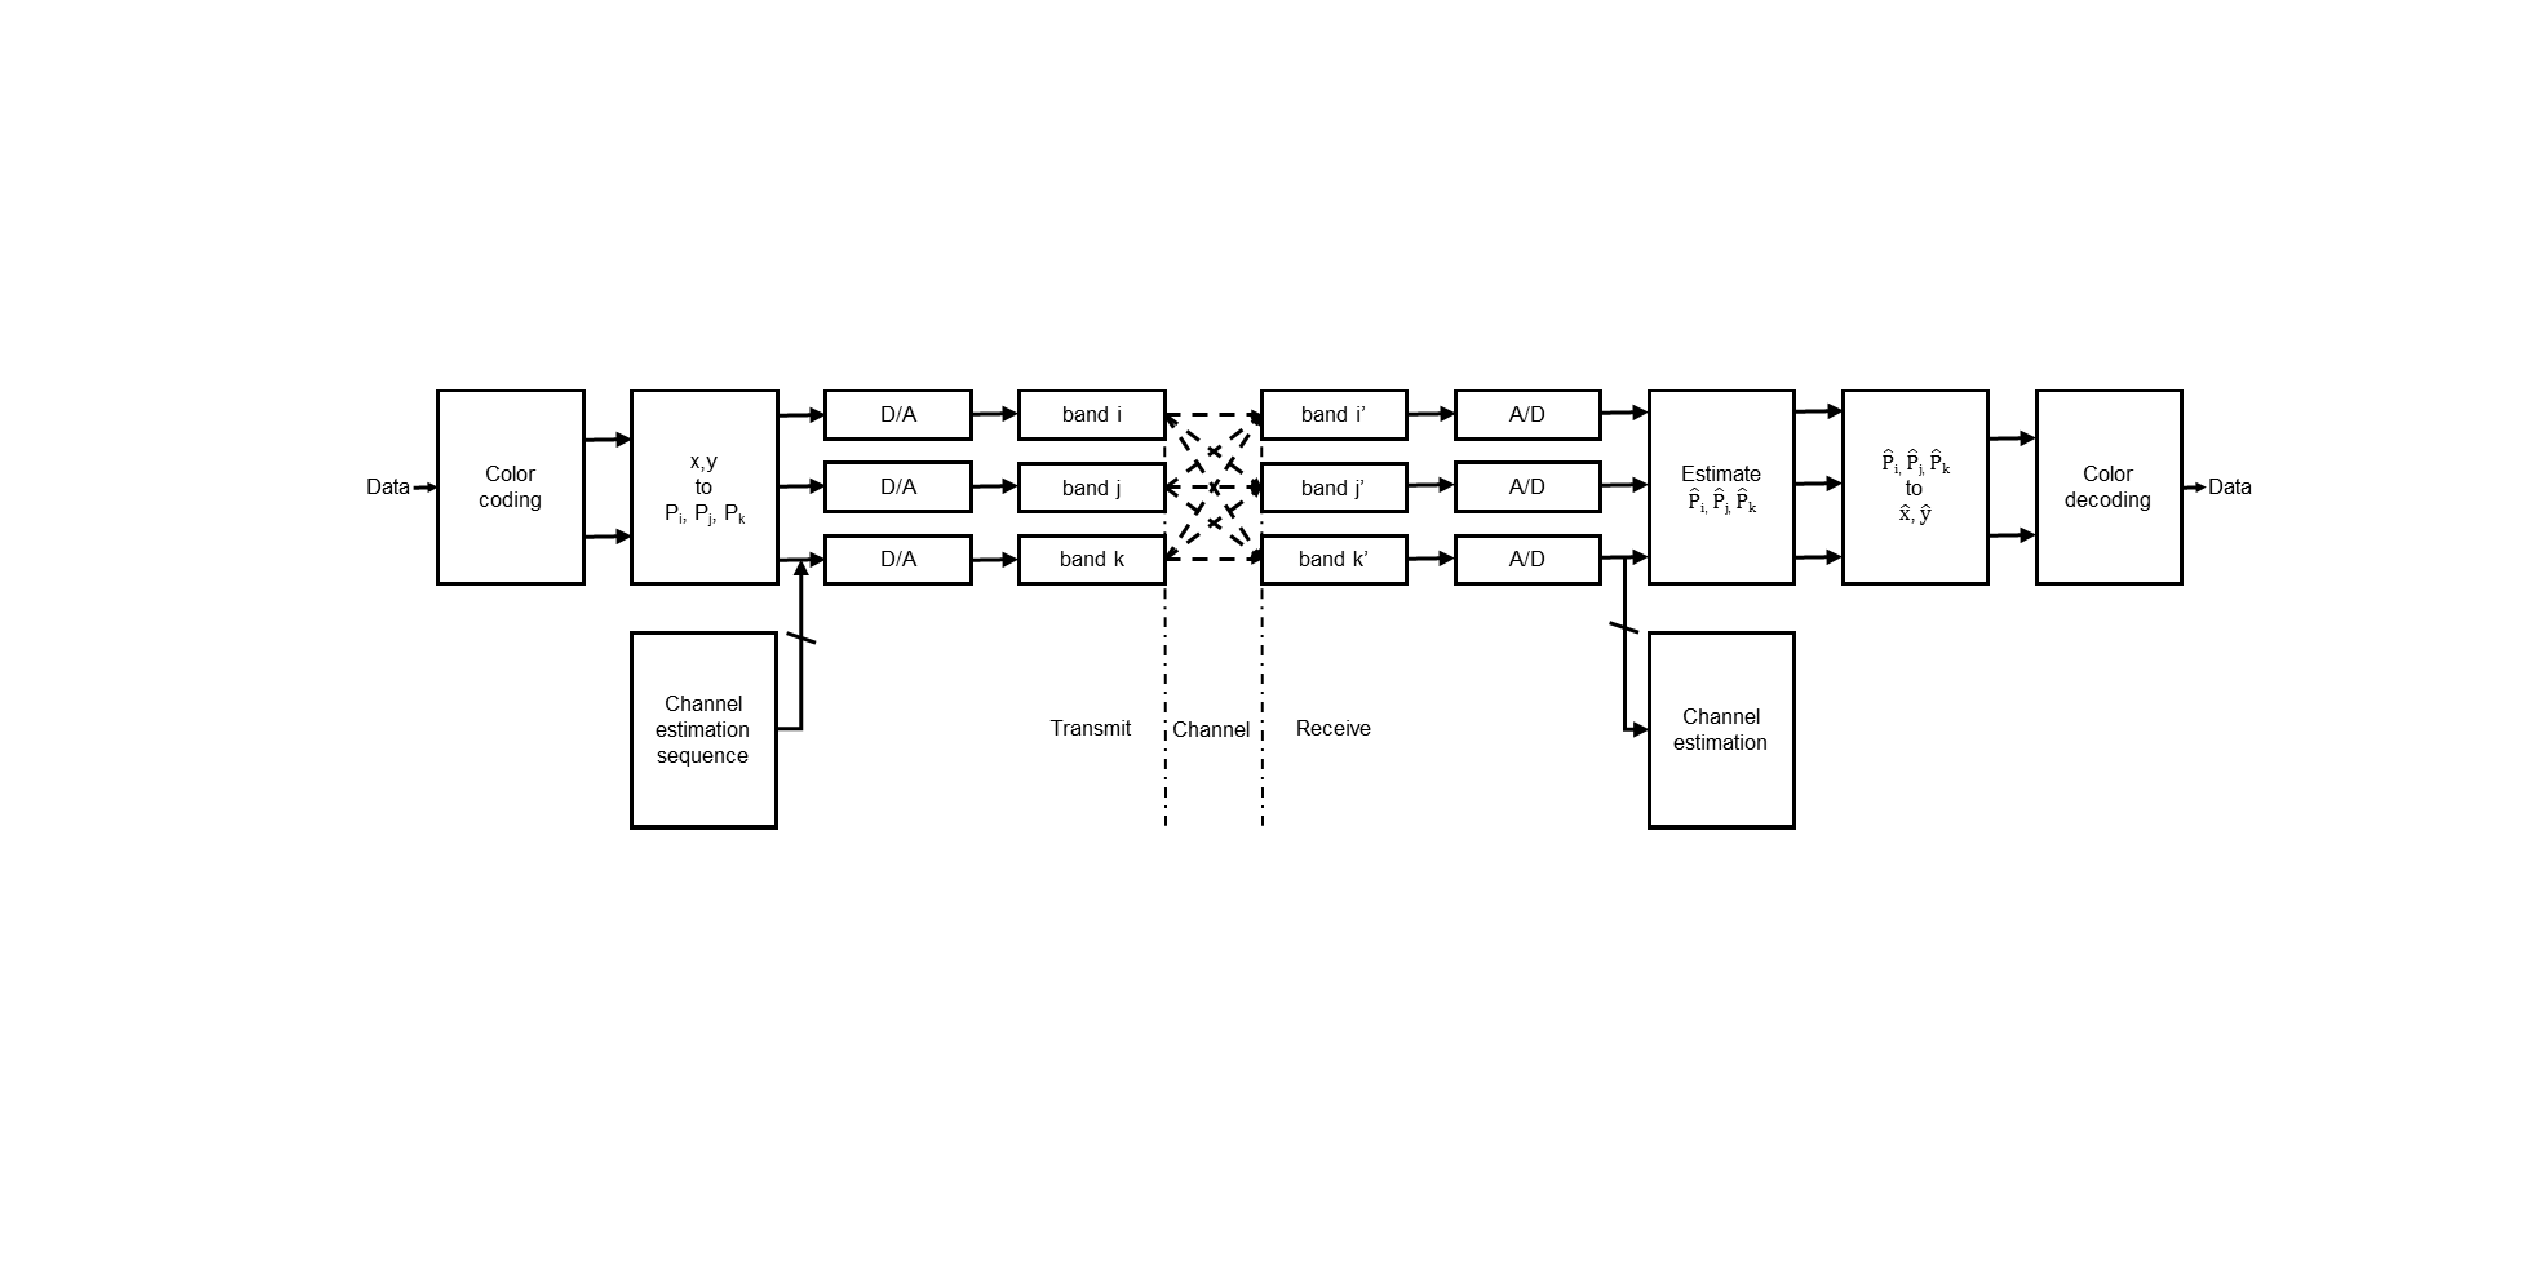
\includegraphics[trim={2.34in 2.78in 1.76in 2.47in}, clip=true, width=5.25in]{CSKBlockDiagram_1.eps}
		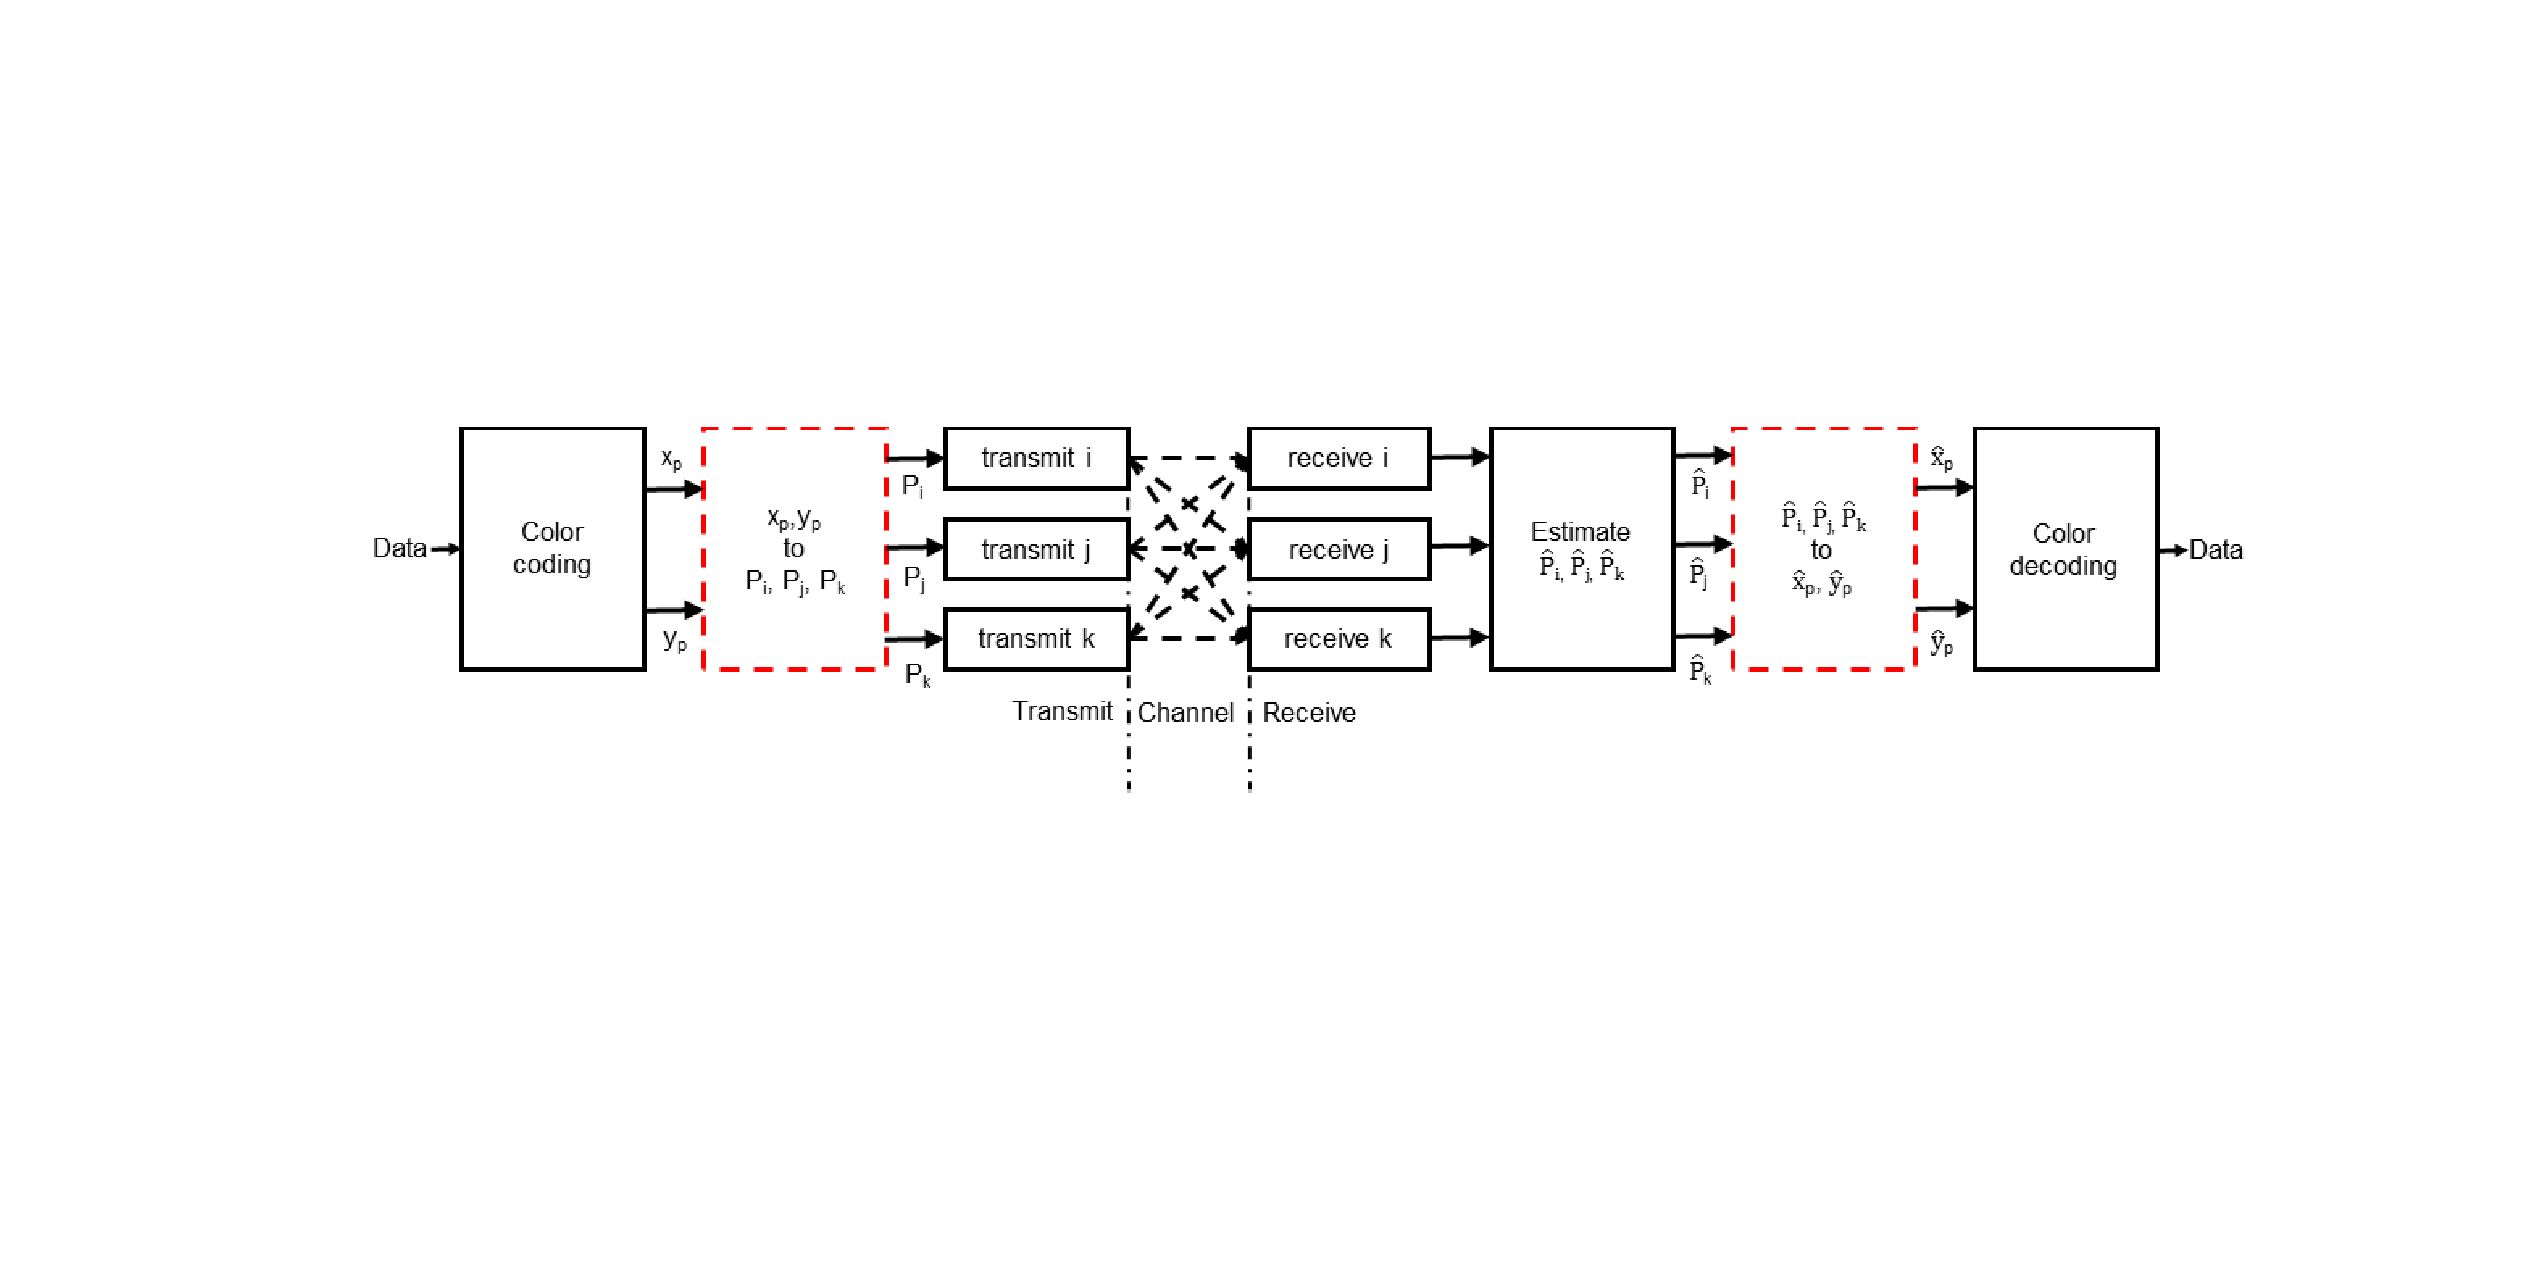
\includegraphics[trim={2.34in 2.78in 1.76in 2.47in}, clip=true, width=5.25in]{CSKBlockDiagram.eps}
	\caption{Block Diagram of CSK Signal Chain.}
	\label{figCSKBD}
\end{figure}

The linear CSK model treats the CIE 1931 XYZ color space as a linear space to analyze CSK performance. This implies the inherent assumption that when irradiance from multiple transmitting elements is combined, the chromaticity coordinates of the resulting SPD is a linear combination of the chromaticity coordinates of the SPDs of individual transmitting elements. If $P_{n}$; $n\in\{i,j,k\}$ is the normalized radiant flux at the transmit or receive device associated with band n, Eq.(\ref{eqLIN}) below taken from reference \cite{ieee802.15.7} provides the mathematical relationships between chromaticity coordinates of all bands and that of resultant SPD.

\begin{equation}
	\begin{aligned}
	x_{p} &= P_{i}x_{i} + P_{j}x_{j} + P_{k}x_{k}\\
	y_{p} &= P_{i}y_{i} + P_{j}y_{j} + P_{k}y_{k}\\
	1 &= P_{i} + P_{j} + P_{k}
\end{aligned}
\label{eqLIN}
\end{equation}

A block diagram of the CSK signaling chain is shown in \figurename\ref{figCSKBD}. At the transmitting element, the data bit-stream is encoded to chromaticity coordinates (x$_p$,y$_p$) to generate an SPD to transmit. Using Eq.(\ref{eqLIN}), normalized $P_{n}$ values are computed which are then scaled to achieve a given illumination target and thus transmit irradiance. Receiving element for band n receives $\hat{P}_{n}$ optical power. Using Eq.(\ref{eqLIN}), the receiver can then estimate transmitted chromaticity coordinates and decode transmitted data.

\begin{figure}[t]
	\centering
		\begin{subfigure}{0.32\textwidth}
		\centering
			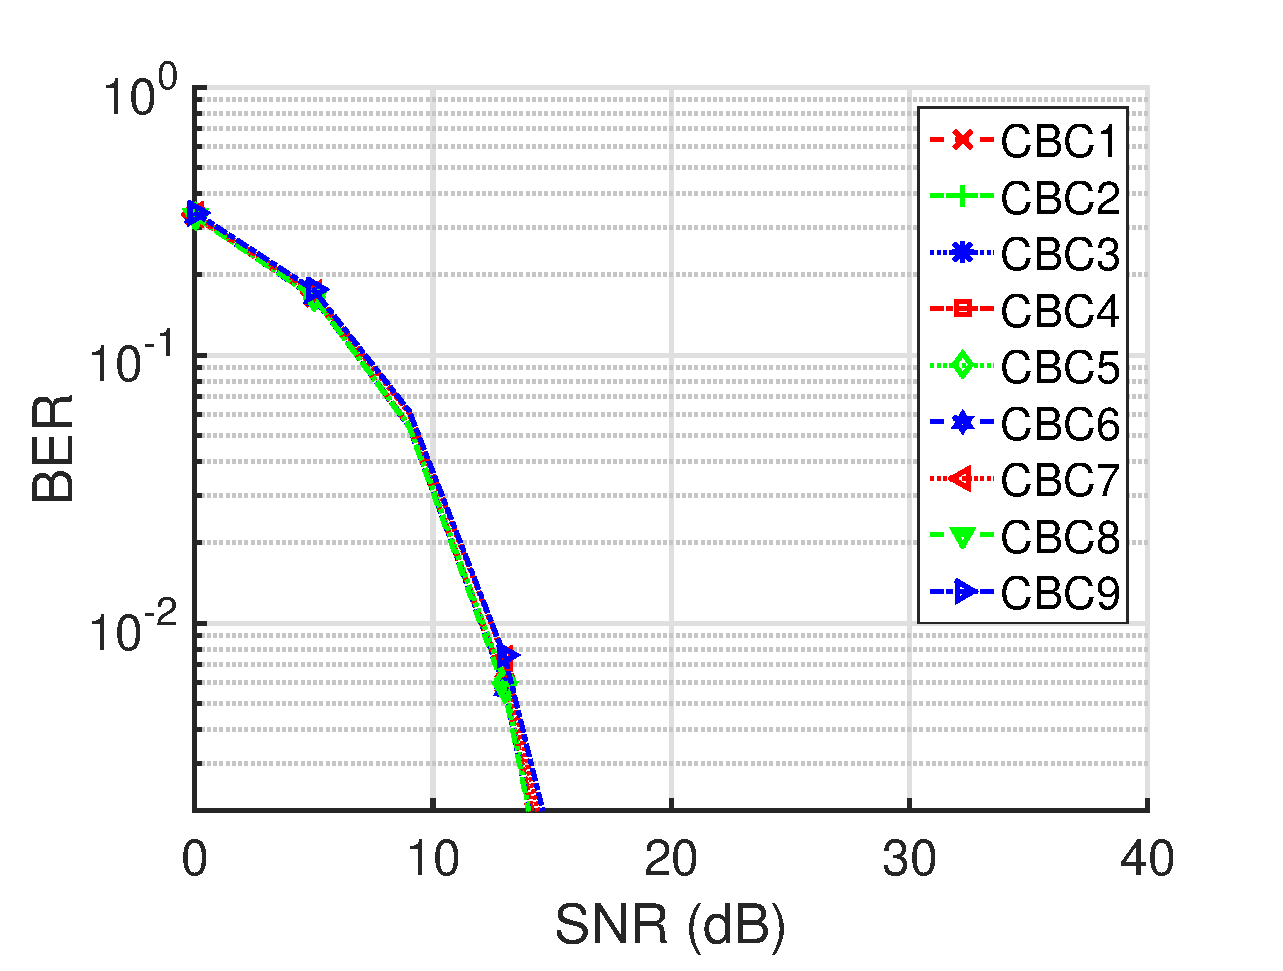
\includegraphics[trim={0.1in 0.0in 0.6in 0.3in}, clip=true, width=\textwidth]{M04_4-CSK_BERvsSNR.eps}
			\caption{4-CSK}
			\label{fig4SNR}
		\end{subfigure}
		\hfill
		\begin{subfigure}{0.32\textwidth}
		\centering
			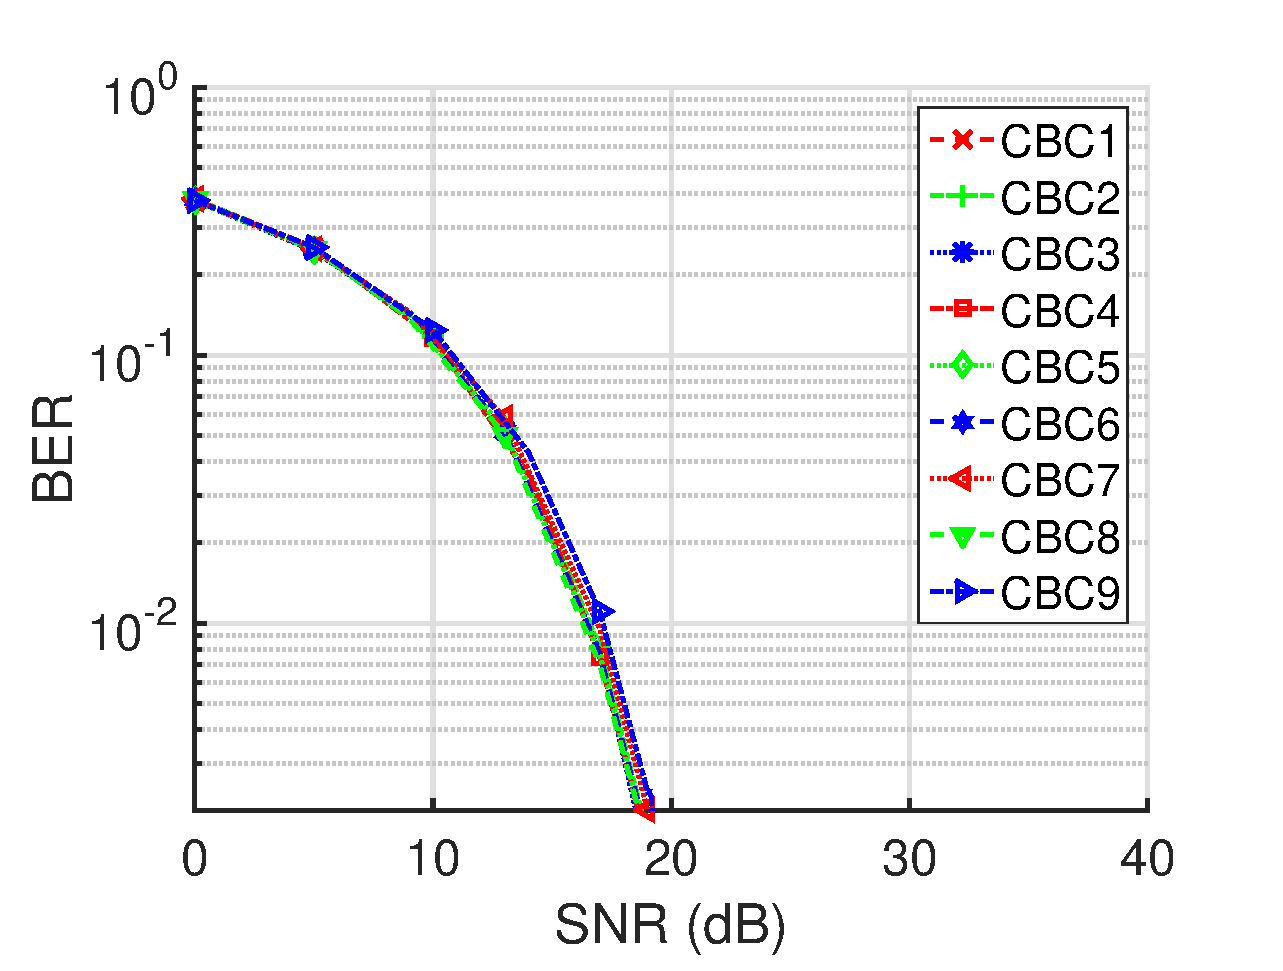
\includegraphics[trim={0.1in 0.0in 0.6in 0.3in}, clip=true, width=\textwidth]{M08_8-CSK_BERvsSNR.eps}
			\caption{8-CSK}
			\label{fig8SNR}
		\end{subfigure}
		\hfill
		\begin{subfigure}{0.32\textwidth}
		\centering
			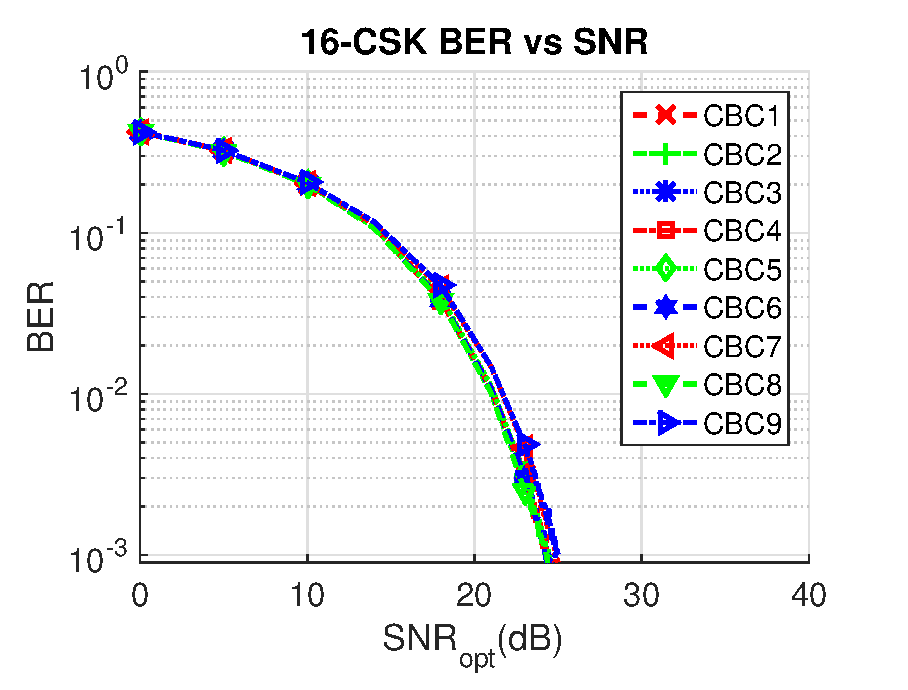
\includegraphics[trim={0.1in 0.0in 0.6in 0.3in}, clip=true, width=\textwidth]{M16_16-CSK_BERvsSNR.eps}
			\caption{16-CSK}
			\label{fig16SNR}
		\end{subfigure}
	\caption{BER vs SNR for linear model}
	\label{figBERvsSNR}
\end{figure}
\begin{figure}[b]
	\centering
		\begin{subfigure}{0.32\textwidth}
		\centering
			\includegraphics[trim={1.0in 0.0in 1.3in 0.1in}, clip=true, width=0.9\textwidth]{M04_4-CSK_CBC2_ReceivedSymbols2.eps}
			\caption{4-CSK}
			\label{fig4RcvSym}
		\end{subfigure}
		\begin{subfigure}{0.32\textwidth}
		\centering
			\includegraphics[trim={1.0in 0.0in 1.3in 0.1in}, clip=true, width=0.9\textwidth]{M08_8-CSK_CBC2_ReceivedSymbols2.eps}
			\caption{8-CSK}
			\label{fig8RcvSym}
		\end{subfigure}
		\begin{subfigure}{0.32\textwidth}
		\centering
			\includegraphics[trim={1.0in 0.0in 1.3in 0.1in}, clip=true, width=0.9\textwidth]{M16_16-CSK_CBC2_ReceivedSymbols3.eps}
			\caption{16-CSK}
			\label{fig16RcvSym}
		\end{subfigure}
		%%%%%%%%% Y0 %%%%%%%%%
		\begin{subfigure}{0.32\textwidth}
		\centering
			\includegraphics[trim={1.0in 0.0in 1.3in 0.1in}, clip=true, width=0.9\textwidth]{M04_4-CSK_CBC2_ReceivedSymbols2_Y0.eps}
			\caption{4-CSK}
			\label{fig4RcvSymY0}
		\end{subfigure}
		\begin{subfigure}{0.32\textwidth}
		\centering
			\includegraphics[trim={1.0in 0.0in 1.3in 0.1in}, clip=true, width=0.9\textwidth]{M08_8-CSK_CBC2_ReceivedSymbols2_Y0.eps}
			\caption{8-CSK}
			\label{fig8RcvSymY0}
		\end{subfigure}
		\begin{subfigure}{0.32\textwidth}
		\centering
			\includegraphics[trim={1.0in 0.0in 1.3in 0.1in}, clip=true, width=0.9\textwidth]{M16_16-CSK_CBC2_ReceivedSymbols3_Y0.eps}
			\caption{16-CSK}
			\label{fig16RcvSymY0}
		\end{subfigure}
	\caption{Received symbols for CBC$_{2}$. (\subref{fig4RcvSym}),(\subref{fig8RcvSym}),(\subref{fig16RcvSym}): Receiver output not clipped. (\subref{fig4RcvSymY0}),(\subref{fig8RcvSymY0}),(\subref{fig16RcvSymY0}): Negative values of receiver output clipped to 0.}
	\label{figRcvSym}
\end{figure}

Monte-carlo simulations are performed to compute performance of M-CSK under the linear model for all CBC$_{v}$. A random bit stream is generated which is then assigned chromaticity coordinates as computed from Table \ref{tMCSK}. As explained before, these are then transformed to $P_{n}$ values. At the receiver, without loss of generality, unity responsivity is assumed. AWGN noise as computed from Eq.\eqref{eqSNR} is then added to each band n. $\hat{P}_{n}$ is then estimated. Using these values, ($\hat{x}_p$,$\hat{y}_p$) are estimated using \eqref{eqLIN}. Maximum likelihood decoder then estimates the transmitted coordinate and recovers the data.

\figurename\ref{figBERvsSNR} shows performance of the 9 CBCs under the linear model. CBC$_{2}$ performs the best whereas CBC$_{9}$ performs the worst. This performance is as expected. As seen from Table \ref{tCBC}, CBC$_{2}$ is composed of CB$_{6}$, CB$_{1}$ and CB$_{0}$ while CBC$_{9}$ is composed of CB$_{2}$, CB$_{1}$ and CB$_{0}$. Thus from values in Table 1 and \figurename 1, it can be seen that constellation points for CBC$_{2}$ are the most spread out and thus have the largest minimum distance between constellation points where as that for CBC$_{9}$ have the shortest spread and thus have the smallest minimum distance between constellation points. SNR of at least 15, 20 and 25 dB are needed to achieve a target minimum bit error rate (BER) of $10^{-3}$ under the linear model for M=4,8,16 CSK respectively.

\figurename\ref{figRcvSym} shows received constellations for CBC$_{2}$ under the linear model. As expected, noise is spread normally along x and y dimensions forming a circular envelop around all constellation points. For M=8 and M=16, 'holes' can be seen in the received coordinates, thus indicating that these constellations could be better packed and further optimized to achieve better spectral efficiency. 

It must be noted here that for \figurename\ref{figRcvSym}(\subref{fig4RcvSym}), (\subref{fig8RcvSym}) and (\subref{fig16RcvSym}), some of the received constellation points are located outside the color gamut (triangle IJK as outlined in \figurename\ref{figConst}) formed by the sources for i,j and k bands. This 'anomaly' can be explained as follows. The CIE 1931 CS is derived assuming (and correctly so) positive radiant fluxes. Under that scenario, the transmitted constellation points reside on or inside the gamut. At the receiver, the unipolar transmitted radiant fluxes are converted into unipolar electrical signal. However this received signal is corrupted by bipolar zero mean Gaussian noise yielding negative receiver output values when negative valued noise dominates over positive valued electrical received signal. If an estimate of transmitted radiant flux is made without first clipping negative valued receiver output to zero, the estimate yields negative flux values. An estimate of transmitted chromaticity coordinates made with these flux values causes some of the estimated constellation points to be located outside the gamut. If the receiver output is clipped to zero, estimated chromaticity coordinates are now illustrated in \figurename\ref{figRcvSym}(\subref{fig4RcvSymY0}), (\subref{fig8RcvSymY0}) and (\subref{fig16RcvSymY0}). The simulation results did not indicate any significant change in performance between the two received signal processing techniques.

While this linear system model is instructive to study CSK modulation and carry out a first order performance analysis, a practical CSK system is non-linear due to non-linearity of the CIE 1931 XYZ space. The (x$_{p}$,y$_{p}$) to P$_{i}$, P$_{j}$, P$_{k}$ block at the transmitter and its counterpart at the receiver (red colored dashed blocks in \figurename\ref{figCSKBD}) introduce this non-linearity which significantly alters the CSK performance for a practical implementation. The effects of these practical constraints on a CSK system are studied in next few sections.

%%%%%%%%%%%%%%%%%%%  Non-linear Model  %%%%%%%%%%%%%%%%%%%%%
\section{CSK: Non-linear system model}\label{sCSKNL}

To understand the source of non-linearity in the CSK system, let's take a look at the CIE 1931 XYZ color space. Let $S_{n}(\lambda)$ be the SPDs of the transmit LEDs and $P_{n}$ be the radiant flux associated with band n. Thus the aggregate transmitted SPD is given by Eq.\eqref{eqWLDA}.

\begin{figure}[b]
	\centering
		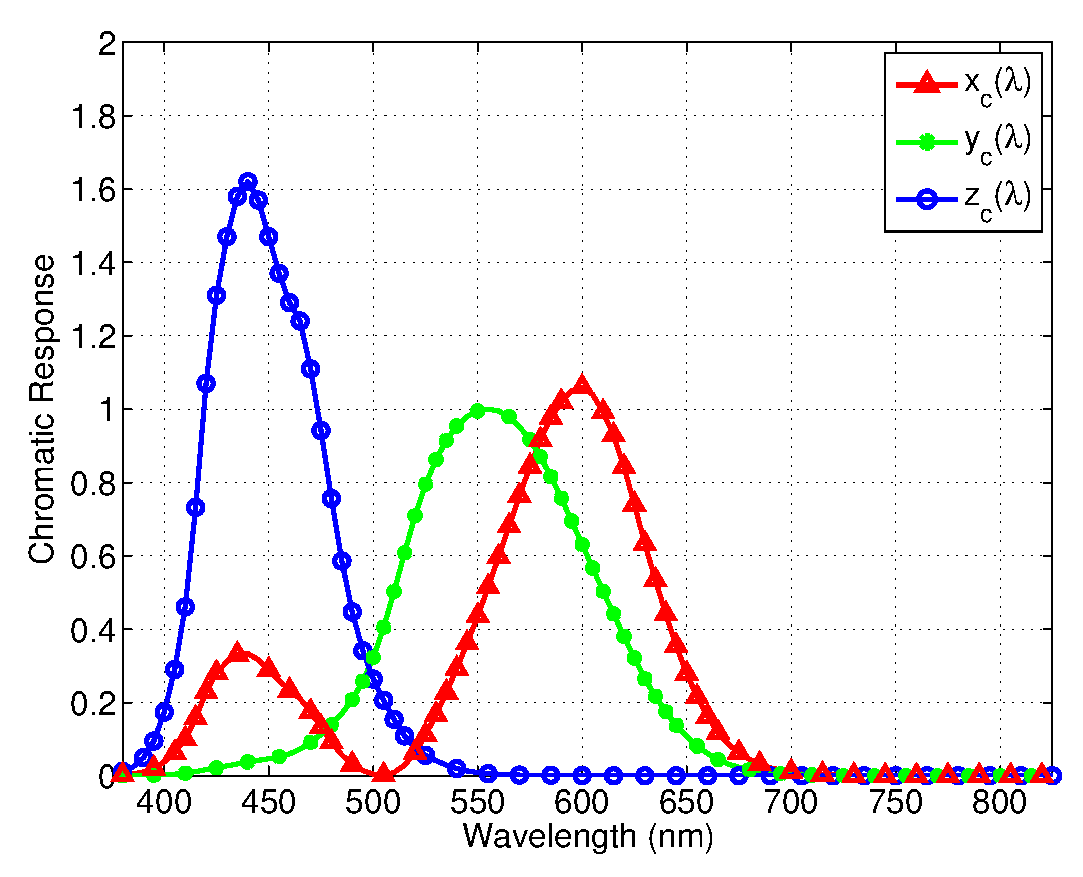
\includegraphics[trim={0.05in 0.05in 0.05in 0.05in}, clip=true, width=2.4in]{CIE1931CMF.eps}
	\caption{CIE 1931 XYZ color matching functions.}
	\label{figCIEXYZ}
\end{figure}

\begin{equation}
	W(\lambda) = \sum\limits_{n\in\{i,j,k\}}P_{n}S_{n}(\lambda)
	\label{eqWLDA}
\end{equation}

CIE 1931 specification outlines three color matching functions - $x_{c}(\lambda)$, $y_{c}(\lambda)$ and $z_{c}(\lambda)$ as illustrated in \figurename\ref{figCIEXYZ}. The tristimulus values for the primaries of CS are given by Eq.\eqref{eqTXYZ} and the chromaticity coordinates (x$_{p}$,y$_{p}$) are given by Eq. \eqref{eqWXY}. 
\begin{equation}
	\begin{aligned}
		X_{W} &= \int\limits_{\lambda=380nm}^{\lambda=780nm}W(\lambda)x_{c}(\lambda)d\lambda\\
		Y_{W} &= \int\limits_{\lambda=380nm}^{\lambda=780nm}W(\lambda)y_{c}(\lambda)d\lambda\\
		Z_{W} &= \int\limits_{\lambda=380nm}^{\lambda=780nm}W(\lambda)z_{c}(\lambda)d\lambda
	\end{aligned}
	\label{eqTXYZ}
\end{equation}

\begin{equation}
	x_{p} = \frac{X_{W}}{X_{W}+Y_{W}+Z_{W}}; \text{  } y_{p} = \frac{Y_{W}}{X_{W}+Y_{W}+Z_{W}} % \text{  } adds space.
	\label{eqWXY}
\end{equation}

\begin{figure}[t]
	\centering
		\begin{subfigure}{0.32\textwidth}
		\centering
			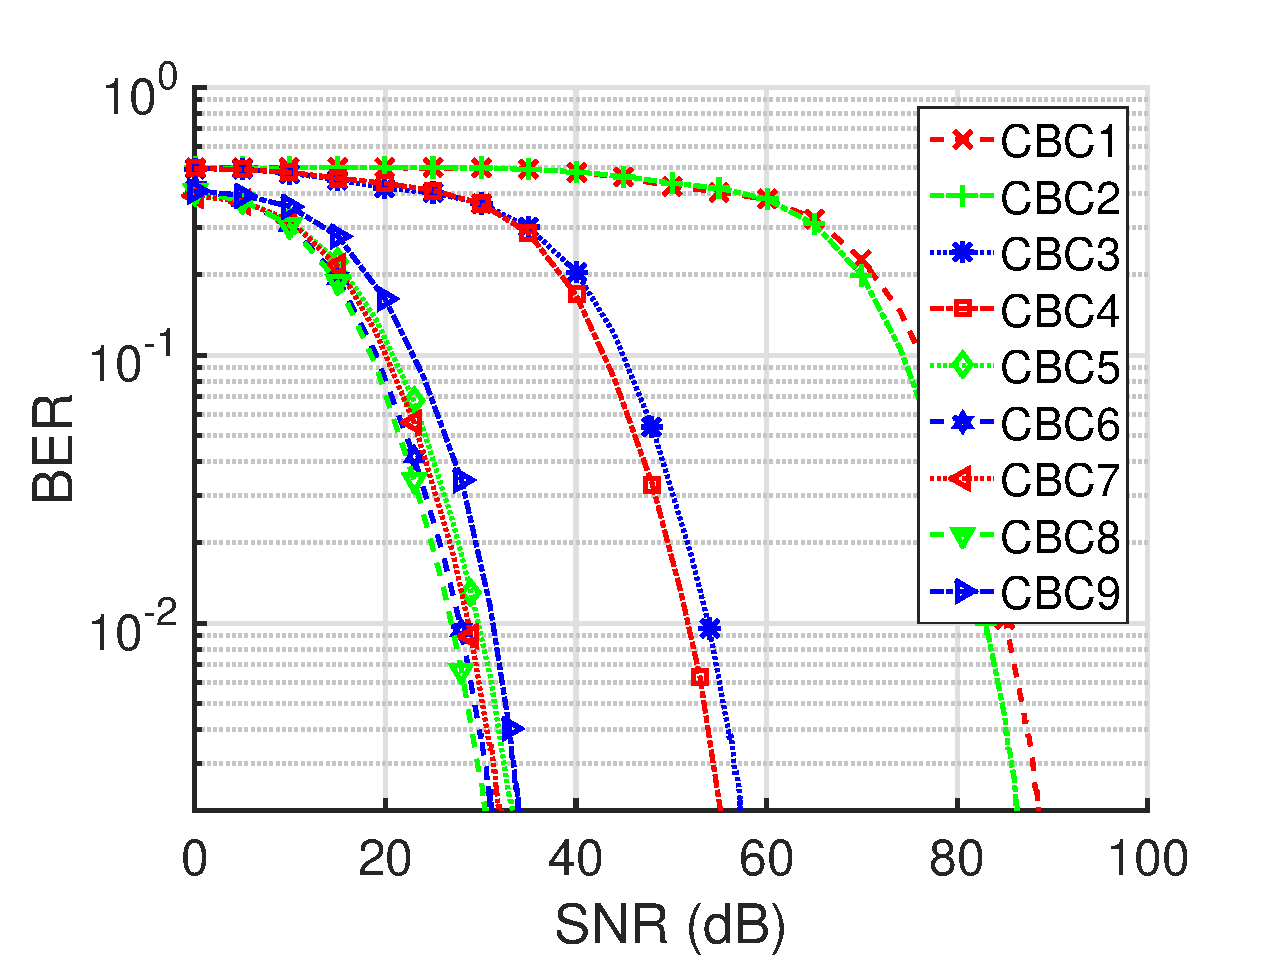
\includegraphics[trim={0.1in 0.0in 0.5in 0.3in}, clip=true, width=\textwidth]{M04_4-CSK_BERvsSNR_NL.eps}
			\caption{4-CSK}
			\label{fig4SNR_NL}
		\end{subfigure}
		\begin{subfigure}{0.32\textwidth}
		\centering
			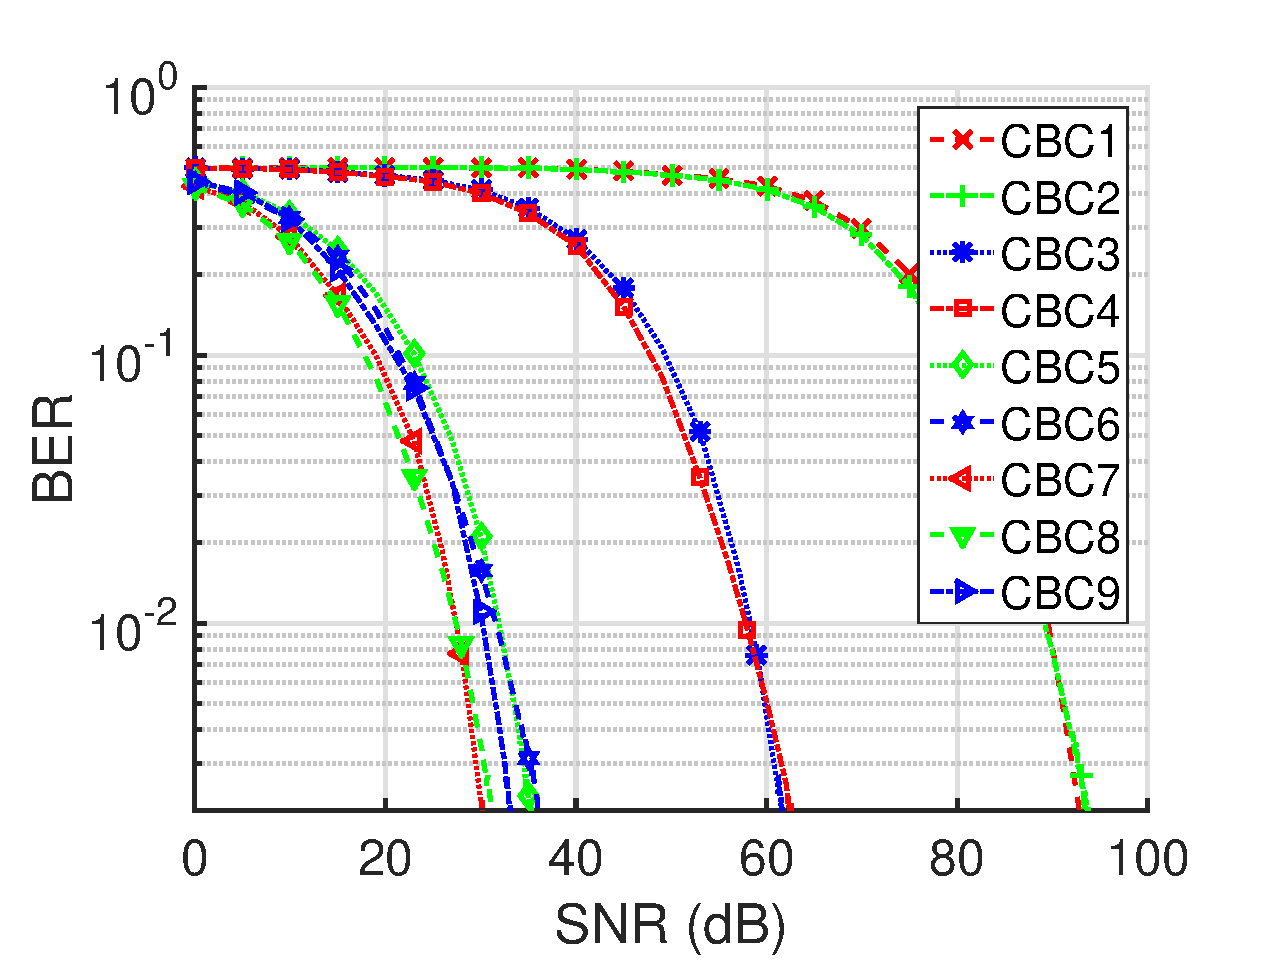
\includegraphics[trim={0.1in 0.0in 0.5in 0.3in}, clip=true, width=\textwidth]{M08_8-CSK_BERvsSNR_NL.eps}
			\caption{8-CSK}
			\label{fig8SNR_NL}
		\end{subfigure}
		\begin{subfigure}{0.32\textwidth}
		\centering
			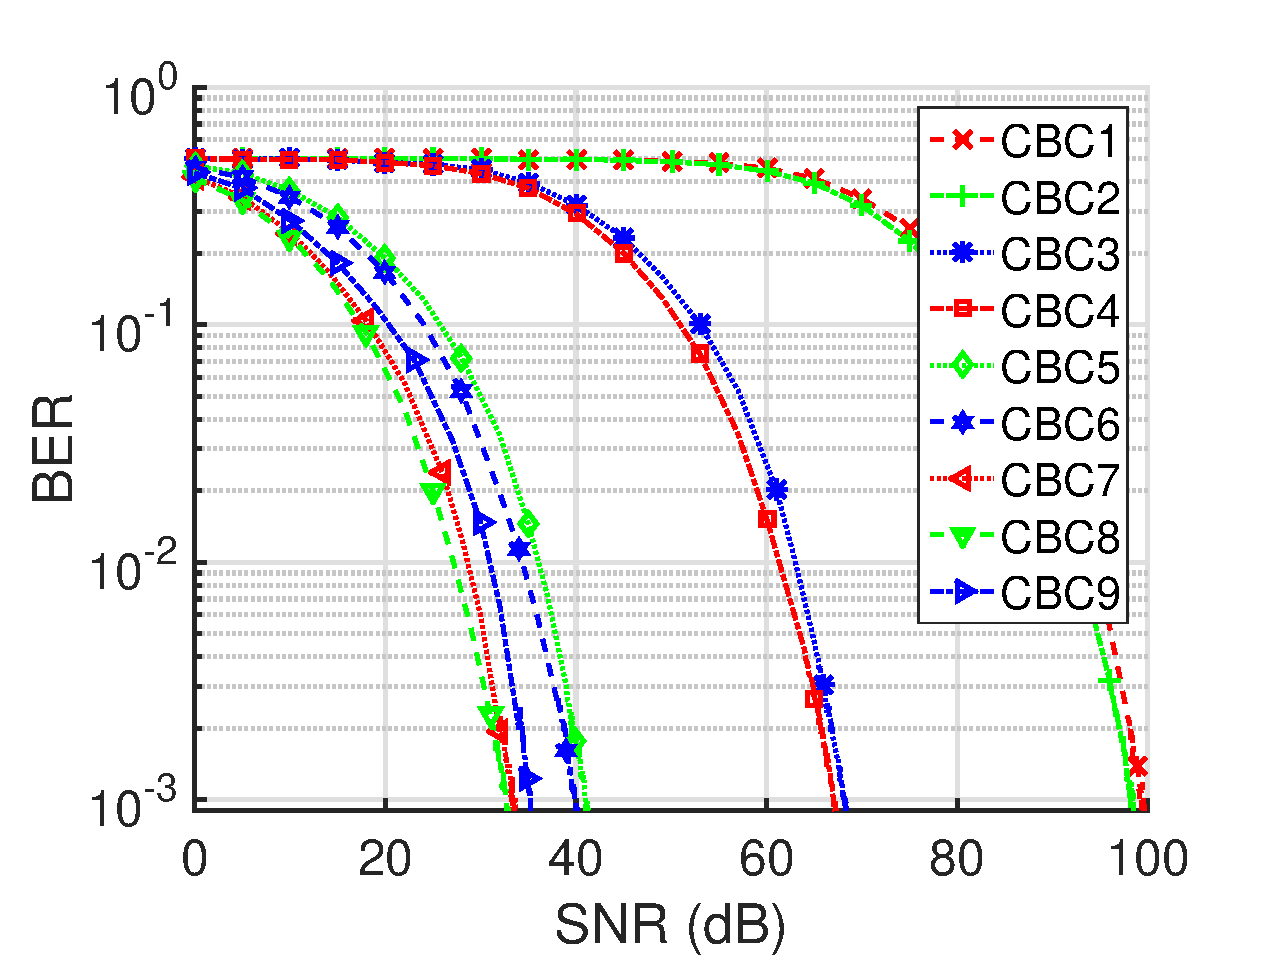
\includegraphics[trim={0.1in 0.0in 0.5in 0.3in}, clip=true, width=\textwidth]{M16_16-CSK_BERvsSNR_NL.eps}
			\caption{16-CSK}
			\label{fig16SNR_NL}
		\end{subfigure}
	\caption{BER vs SNR for all CBC}
	\label{figBERvsSNR_NL}
\end{figure}

\begin{figure}[b]
	\centering
		\begin{subfigure}{0.32\textwidth}
		\centering
			\includegraphics[trim={1.0in 0.0in 1.3in 0.1in}, clip=true, width=\textwidth]{M04_4-CSK_CBC1_ReceivedSymbols9_NL.eps}
			\caption{CBC$_{1}$: 4-CSK}
			\label{fig4RcvSym_NL}
		\end{subfigure}
		\begin{subfigure}{0.32\textwidth}
		\centering
			\includegraphics[trim={1.0in 0.0in 1.3in 0.1in}, clip=true, width=\textwidth]{M08_8-CSK_CBC1_ReceivedSymbols10_NL.eps}
			\caption{CBC$_{1}$: 8-CSK}
			\label{fig8RcvSym_NL}
		\end{subfigure}
		\begin{subfigure}{0.32\textwidth}
		\centering
			\includegraphics[trim={1.0in 0.0in 1.3in 0.1in}, clip=true, width=\textwidth]{M16_16-CSK_CBC1_ReceivedSymbols10_NL.eps}
			\caption{CBC$_{1}$: 16-CSK}
			\label{fig16RcvSym_NL}
		\end{subfigure}
		%%%%%%%%% CBC8 %%%%%
		\begin{subfigure}{0.32\textwidth}
		\centering
			\includegraphics[trim={1.0in 0.0in 1.3in 0.1in}, clip=true, width=\textwidth]{M04_4-CSK_CBC8_ReceivedSymbols4_NL.eps}
			\caption{CBC$_{8}$: 4-CSK}
			\label{fig4RcvSym_NL8}
		\end{subfigure}
		\begin{subfigure}{0.32\textwidth}
		\centering
			\includegraphics[trim={1.0in 0.0in 1.3in 0.1in}, clip=true, width=\textwidth]{M08_8-CSK_CBC8_ReceivedSymbols4_NL.eps}
			\caption{CBC$_{8}$: 8-CSK}
			\label{fig8RcvSym_NL8}
		\end{subfigure}
		\begin{subfigure}{0.32\textwidth}
		\centering
			\includegraphics[trim={1.0in 0.0in 1.3in 0.1in}, clip=true, width=\textwidth]{M16_16-CSK_CBC8_ReceivedSymbols4_NL.eps}
			\caption{CBC$_{8}$: 16-CSK}
			\label{fig16RcvSym_NL8}
		\end{subfigure}
	\caption{Received symbols for non-linear model.}
	\label{figRcvSym_NL}
\end{figure}

As outlined in prior sections, M-ary CSK modulation transmits information by varying the chromaticity coordinates of transmit SPD. In a practical implementation, a table of unique transformation ratios $P_{i}$:$P_{j}$:$P_{k}$ $\rightarrow$ $(x_{p},y_{p})$ can be pre-computed. Referring back to \figurename\ref{figCSKBD}, at the transmitter the data is color coded to obtain $(x_{p},y_{p})$ coordinate to transmit. Given this coordinate, corresponding flux ratios $P_{i}$:$P_{j}$:$P_{k}$ can be looked up from the pre-computed table. The target illumination requirements provide the total radiant flux to output from the transmitter. With this information, individual $P_{n}$ for each band n can now be computed from Eq. \eqref{eqWLDA}. It can also be inferred that the relationship between $P_{n}$ and (x$_{p}$,y$_{p}$) is non-linear.

From the channel model in Eq.\eqref{eqCHNL} it can be seen that AWGN gets added to received signal which is then used to compute an estimate of transmitted radiant fluxes $\hat{P}_{n}$. Eqs.(\ref{eqWLDA}-\ref{eqWXY}) can then be used to estimate transmitted coordinate ($\hat{x}_{p}$,$\hat{y}_{p}$). Thus, the additive noise undergoes a non-linear transformation during $\hat{P}_{n}\rightarrow$ ($\hat{x}_{p}$,$\hat{y}_{p}$) which skews the noise in the chromaticity plane. This causes additional performance penalties in a practical system.

\figurename\ref{figBERvsSNR_NL} shows performance of all the CBCs under this non-linear model. These curve are obtained by monte-carlo simulations similar to those performed for the linear model after substituting the $P_{n}$ $\rightarrow$ (x$_{p}$,y$_{p}$) and $\hat{P}_{n}\rightarrow$ ($\hat{x}_{p}$,$\hat{y}_{p}$) with the non-linear system model transformations. It can be observed that CBC$_{8}$ performs the best while CBC$_{1}$ performs the worst. Additionally, it is observed that CBC$_{1}$-CBC$_{4}$ perform significantly worse as compared to the rest. For CBC$_{1}$-CBC$_{4}$, the amount of radiant flux emitted by band i is 3-4 orders of magnitude greater than band j and 1-2 orders of magnitude greater than band k. Thus the $\hat{P}_{n}\rightarrow (\hat{x}_{p},\hat{y}_{p})$ conversion at the receiver is extremely sensitive to noise along the j and k bands as compared to that along i band. This introduces significant errors in decoding received symbols closer to the i band.

\figurename\ref{figRcvSym_NL} shows received constellation for CBC$_{1}$ and CBC$_{8}$ under the non-linear model. Noise skew about the estimated coordinates can be observed here. This noise skew is more prominent for CBC$_{1}$ where the signal power distribution along all bands is imbalanced as compared to that for CBC$_{8}$ where signal power is more uniformly spread across all bands. It can be seen that AWGN introduced on P$_{n}$, gets skewed radially towards band k due to non-linearity in $P_{n}\rightarrow (x,y)$ transformation and is no longer AWGN along the (x,y) chromaticity plane. This generates an interesting outcome in that for CBC$_{8}$, about 30dB of SNR is needed to achieve target $10^{-3}$ BER for all of M = 4,8,16 CSK. This happens because with increase in order M, the additional constellation points as defined in the standard happen to occupy non-interfering regions of the chromaticity plane thus increasing spectral efficiency without incurring any SNR penalty up to a point. The non-linearity of the CIE 1931 XYZ space introduces performance penalties of at least 15dB, 10dB and 5dB for M = 4,8,16 CSK respectively over CBC$_{2}$ used in linear system model.

%%%%%%%%%%%%%%%%%%%%%  Illumination  %%%%%%%%%%%%%%%%%%%%%%%
\section{CSK: Performance under illumination constraints}\label{sCSKLSNR}

%%%%%%%%%%%%  Luminous Signal to Noise Ratio  %%%%%%%%%%%%%%
\subsection{Luminous signal-to-noise ratio}\label{ssLSNR}

In an indoor optical wireless system using lighting devices for wireless downlink access the luminaires need to simultaneously service illumination and optical wireless broadcast missions. Under this model, different colored PHY (example: different CBC$_{v}$) irradiate different amounts of radiant flux to achieve the same illumination intensity level. Thus, it is unfair to use SNR as a metric to compare performance of modulation schemes at same BER target using different colored PHY without first normalizing for illumination targets. Thus, in this section we introduce luminous-signal-to-noise ratio (LSNR) as a metric that takes into account the differences in radiant flux emitted by different PHY to achieve the same illumination intensity level.

Consider optical modulation scheme(s) which can be implemented with two different constellations C$_a$ or C$_b$. The fluxes emitted by the two constellations are scaled to achieve a target illumination intensity level. Let both constellations on average emit I lumens of luminous flux. Let the luminous efficacy for the two constellations be specified by $\eta_a$ and $\eta_b$ in lumens-per-watt respectively. Then the corresponding average radiant flux emitted by the two constellations is given by W$_a$ = I/$\eta_a$ and W$_b$  = I/$\eta_b$ watts respectively. 

Let us define a luminous ratio L$_{ab}\triangleq (\eta_a/\eta_b) \equiv$ (W$_b$/W$_a$). Thus, for every 1 Watt of radiant flux emitted by C$_a$, C$_b$ must emit L$_{ab}$ Watt of radiant flux to achieve the same illumination intensity level. Under the model where the luminaires service illumination along with communication, it is fair to compare the performance of the two schemes at these \textit{relative} radiant flux levels instead of at the absolute radiant flux levels. Thus we define the LSNR metric in Eq.\eqref{eqLSNR} as a means to compare performance of C$_b$ versus that of C$_a$ at same illumination levels. 

\begin{equation}
	% ^{ } is used with \vm{X} to help align subscript 'b' for both \vm{X} below.
	LSNR_{ab} \triangleq \frac{\text{L}^{2}_{ab}Tr\{\vm{H}\vm{X}^{ }_{b}\vm{X}^{*}_{b}\vm{H}^{*}\}}{\sigma^{2}_{n}} 
	\label{eqLSNR}
\end{equation}
where \vm{X}$_{b}$ is the average radiant flux emitted by C$_b$. Thus, after computing BER vs SNR for the scheme employing C$_a$, BER vs LSNR can be computed for scheme employing C$_b$ to compare its performance \textit{relative} to that employing C$_a$ at the same illumination levels.

%%%%%%%%%%%%%%%%%%%%%  Illumination  %%%%%%%%%%%%%%%%%%%%%%%
\subsection{Performance under illumination constraints}\label{ssCSKLSNR}

\begin{figure}[t]
	\centering
		\begin{subfigure}{0.32\textwidth}
		\centering
			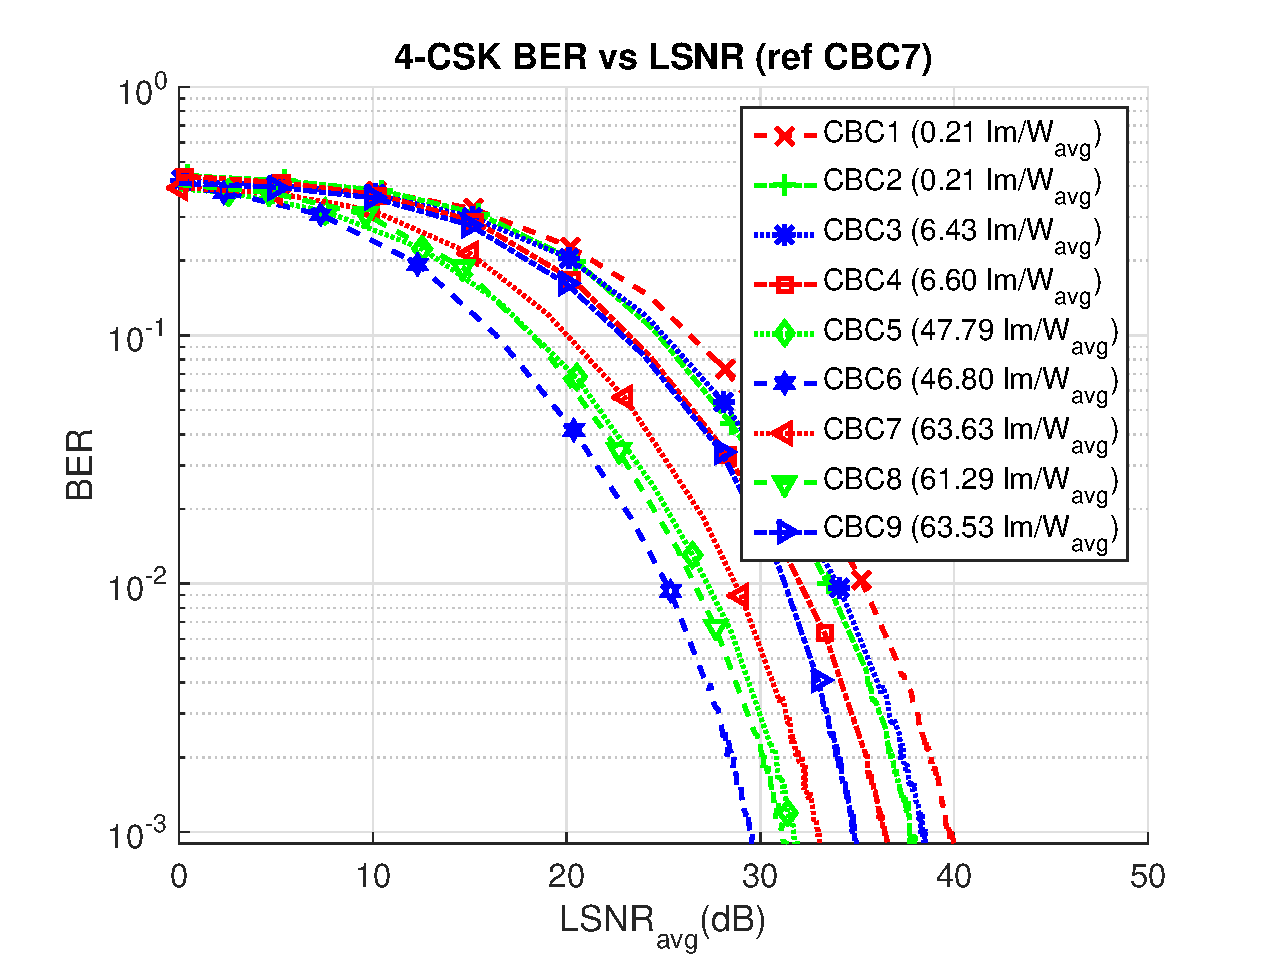
\includegraphics[trim={0.1in 0.0in 0.5in 0.1in}, clip=true, width=\textwidth]{M04_4-CSK_BERvsLSNR_NL.eps}
			\caption{4-CSK}
			\label{fig4LSNR}
		\end{subfigure}
		\begin{subfigure}{0.32\textwidth}
		\centering
			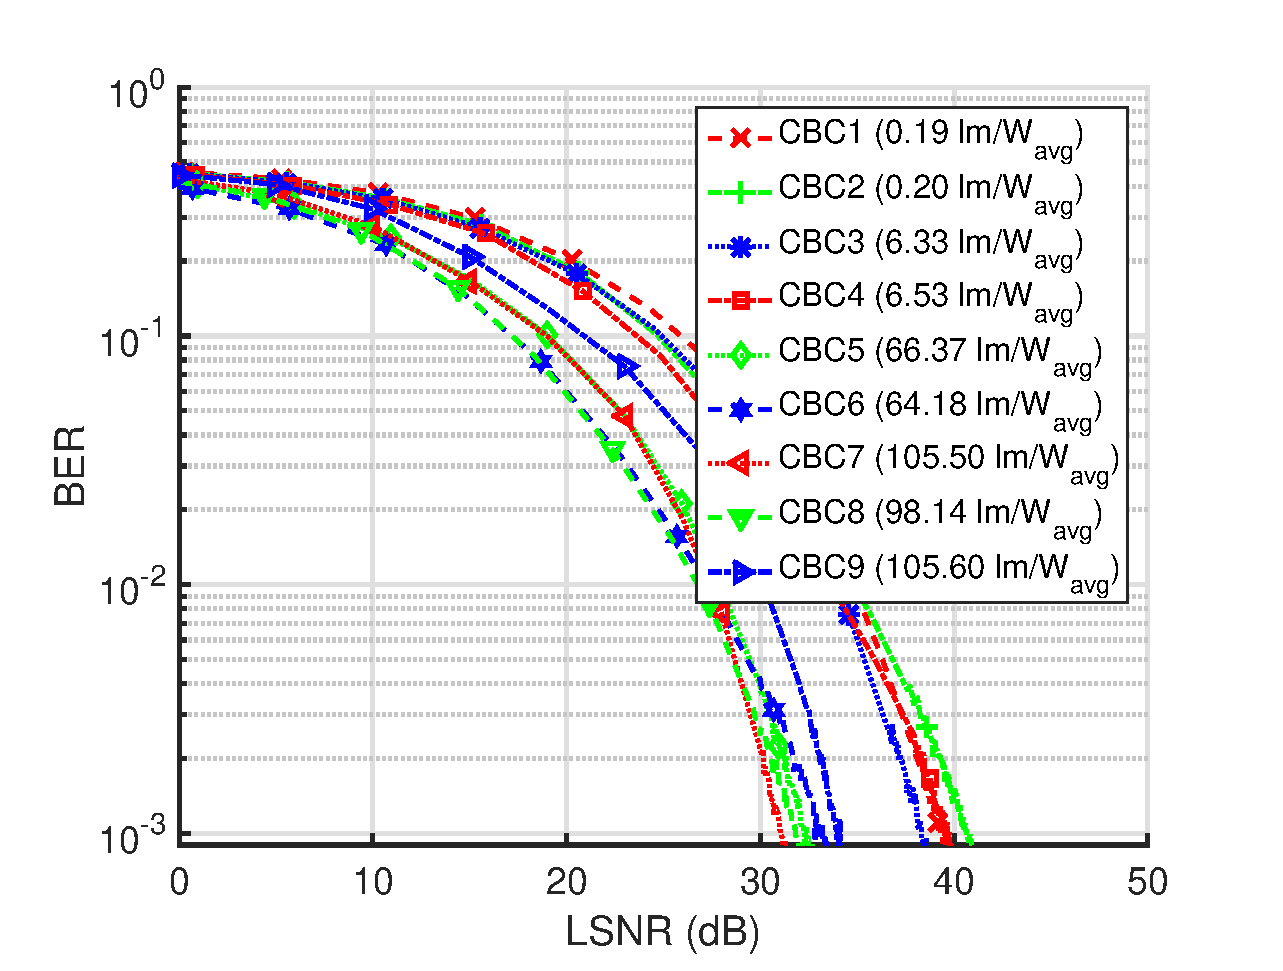
\includegraphics[trim={0.1in 0.0in 0.5in 0.1in}, clip=true, width=\textwidth]{M08_8-CSK_BERvsLSNR_NL.eps}
			\caption{8-CSK}
			\label{fig8LSNR}
		\end{subfigure}
		\begin{subfigure}{0.32\textwidth}
		\centering
			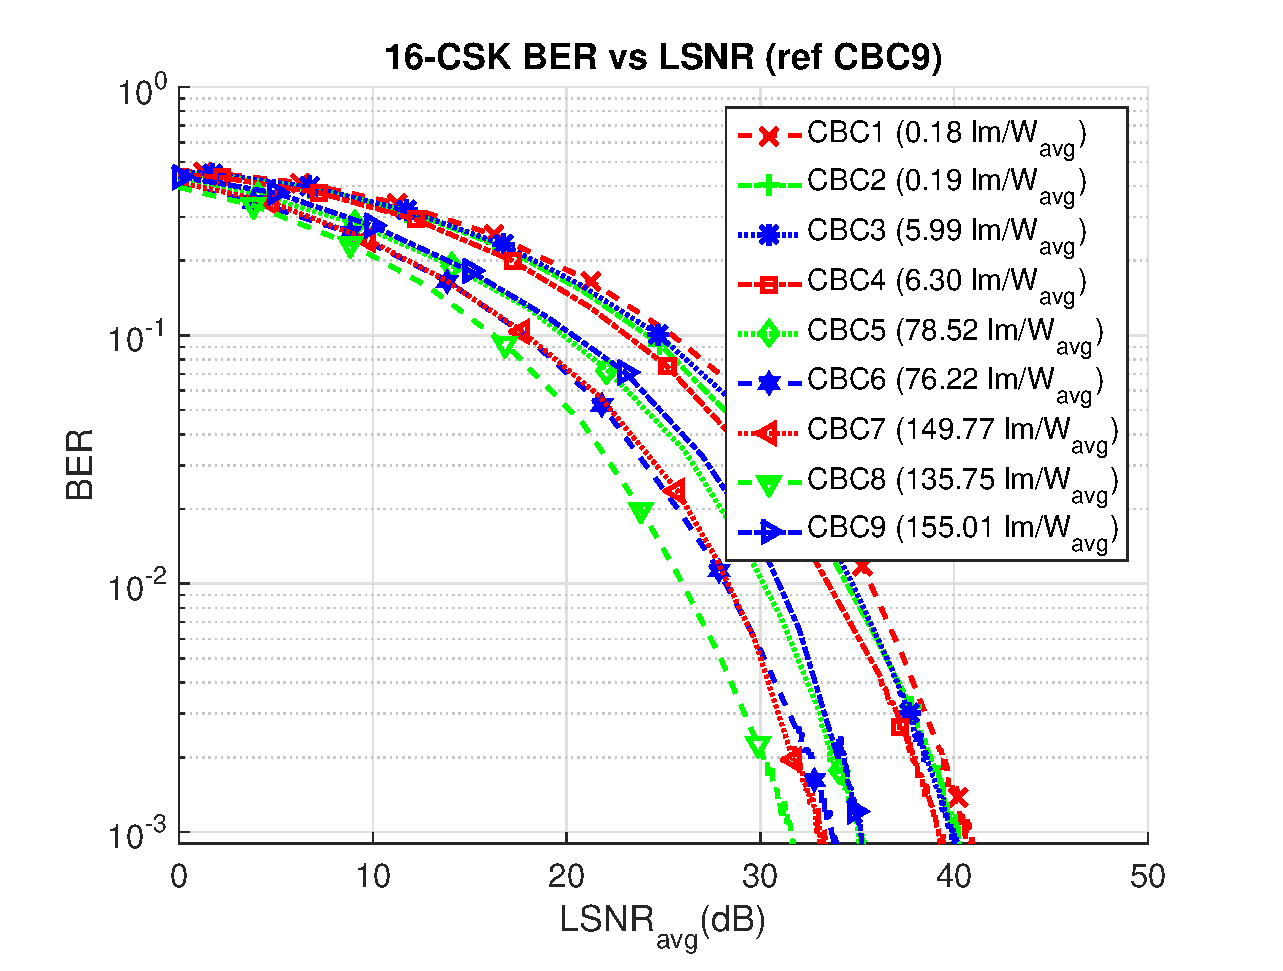
\includegraphics[trim={0.1in 0.0in 0.5in 0.1in}, clip=true, width=\textwidth]{M16_16-CSK_BERvsLSNR_NL.eps}
			\caption{16-CSK}
			\label{fig16LSNR}
		\end{subfigure}
	\caption{BER vs LSNR for all CBC}
	\label{figBERvsLSNR}
\end{figure}

\figurename\ref{figBERvsLSNR} shows performance of the 9 CBCs under the non-linear model when normalized for illumination constraints. The efficacies of all CBC for different M are specified in the legends. These values are used to normalize the performance of M-CSK for all CBC using CBC with highest efficacy as the reference for LSNR calculation. The effect of this is to shift all curves from \figurename\ref{figBERvsSNR_NL} towards left along the x-axis depending on the L$_{ab}$ values in Eq.\eqref{eqLSNR}. It can be observed that given a target illumination intensity level, CBC$_{6}$ performs the best for 4-CSK while CBC$_{8}$ performs the best for 8-CSK and 16-CSK. For CBC$_{1}$-CBC$_{4}$, due to their low luminous efficacy, one can use a much larger radiant flux to achieve target illumination levels and thus significantly improve their communication performance. However, this is achieved at the cost of poor energy efficiency. In contrast, CBC$_{7}$ and CBC$_{9}$ have relatively high luminous efficacy. This implies that these CBCs are restricted to emit a relatively low radiant flux (and thus low signal powers) to achieve target illumination level. Thus despite being relatively energy efficient for illumination purpose, these CBCs suffer from relatively poor communication performance.

%%%%%%%%%%%%%%%%%%%%%%  Conclusion  %%%%%%%%%%%%%%%%%%%%%%%%
\section{Conclusion}\label{sCONC}
This article studies performance of all CBCs as specified in reference \cite{ieee802.15.7}. Under the linear system model CBC$_{2}$ performs the best and needs SNR of at least 15dB, 20dB and 25dB to achieve target BER = $10^{-3}$ for M=4,8,16-CSK respectively. The non-linear system model is then considered and it is shown that the non-linearity of the CIE 1931 XYZ color space implies that the AWGN introduced to the received signal gets skewed and is no longer AWGN when transformed to the chromaticity plane. Under the non-linear system model, CBC$_{8}$ performs the best with a performance penalty of at least 15dB, 10dB and 5dB for over CBC$_{2}$ in linear model for M = 4,8,16-CSK respectively. The article then introduces LSNR metric to compare performance of any two signaling schemes using the visible spectrum after normalizing signal powers (radiant flux) to achieve a target illumination intensity level. Performance comparisons of M-ary CSK for all CBCs then reveal that CBC$_{6}$ performs the best for 4-CSK while CBC$_{8}$ performs the best for 8-CSK and 16-CSK. 

Optimal performance of CSK can be seen as a tradeoff between the illumination and communication missions. There is further scope to optimize the M-ary CSK constellations under the practical non-linear model by selecting optical sources centered at different wavelengths than those considered in the standard. After characterizing skew for AWGN along the chromaticity plane, constellation points can be optimally positioned to further improve the M-ary CSK performance.

%%%%%%%%%%%%%%%%%%%%  Acknowledgment  %%%%%%%%%%%%%%%%%%%%%%
\section*{Acknowledgment}
This work was supported by the Engineering Research Centers Program of the National Science Foundation under NSF Cooperative Agreement No. EEC-0812056.

\end{document}
